\documentclass[11pt]{article}
\usepackage[T1]{fontenc}
\usepackage[utf8]{inputenc}
\usepackage{lmodern}
\usepackage[margin=1in]{geometry}
\usepackage{amsmath,amssymb,amsthm,mathtools,bm}
\usepackage{longtable,booktabs,array}
\usepackage[shortlabels]{enumitem}
\usepackage{hyperref}
\usepackage{xurl}
\usepackage{tikz}
\usetikzlibrary{arrows.meta,positioning,calc}

\hypersetup{colorlinks=true,linkcolor=blue,citecolor=blue,urlcolor=blue}
\setlength{\emergencystretch}{3em}
\renewcommand{\arraystretch}{1.08}
\newcolumntype{L}[1]{>{\raggedright\arraybackslash}p{#1}}

\newtheorem{theorem}{Theorem}[section]
\newtheorem{proposition}[theorem]{Proposition}
\newtheorem{definition}[theorem]{Definition}
\newtheorem{assumption}[theorem]{Assumption}
\newtheorem{conjecture}[theorem]{Conjecture}
\newtheorem{claim}[theorem]{Claim}
\newtheorem{postulate}[theorem]{Postulate}
\theoremstyle{remark}
\newtheorem{remark}[theorem]{Remark}
\theoremstyle{plain}

\newcommand{\OPH}{\mathrm{OPH}}
\newcommand{\A}{\mathbb A}
\newcommand{\R}{\mathbb R}
\newcommand{\E}{\mathbb E}
\newcommand{\TV}{\mathrm{TV}}
\newcommand{\rec}{\mathrm{rec}}
\newcommand{\bd}{\partial}
\newcommand{\diag}{\mathrm{diag}}
\newcommand{\anti}{\mathrm{anti}}
\newcommand{\erank}{\mathrm{erank}}
\newcommand{\argmax}{\operatorname*{arg\,max}}
\newcommand{\argmin}{\operatorname*{arg\,min}}

\title{Thinking as Patch-Net Fixed-Point Search:\\
A Mathematical Model of Neural Consensus Computation}
\author{B.\ M\"uller}
\date{Draft of May 7, 2026}
\newcommand{\OPHPaperReleaseID}{r1520}
\newcommand{\OPHPaperReleaseDate}{July 9, 2026}
\newcommand{\OPHPaperReleaseBanner}{%
\begin{center}
\small\textbf{Paper release:} \texttt{\OPHPaperReleaseID}\quad\textbf{Released:} \OPHPaperReleaseDate
\end{center}
}


\begin{document}
\maketitle
\begin{center}
\small\textbf{Paper release:} \OPHPaperReleaseID\quad
\textbf{Released:} \OPHPaperReleaseDate
\end{center}

\begin{abstract}
Thinking can be modeled as patch-net fixed-point search. A thought is a trajectory through feedback local patches. An insight, percept, decision, or remembered meaning is the stable form reached after enough mismatch has been repaired.

The same mechanism can be read across substrates. Finite patches expose boundary readouts, compare overlaps, and settle by accepted repair moves. Brains may approximate this machine through feedback neural dynamics, dendritic integration, oscillations, inhibition, plasticity, body state, and action feedback. The hardware comparison is the Echosahedron, used as a controllable self-reading patch. Across substrates the same vocabulary applies: patch data, transition, self-read, repair, record, fixed point.
\end{abstract}

\section*{What This Paper Contributes}

The paper imports familiar pieces from neuroscience and computation: recurrent
networks, predictive coding, attractor dynamics, dendritic integration,
oscillation, inhibition, plasticity, body state, and action feedback. OPH adds
one discipline to that list. A thought is treated as an observer-facing normal
form reached by local mismatch repair in a self-reading patch federation.

That gives a common language for brains, OPH observer patches, and the
Echosahedron hardware comparison. The claim is conditional: a biological
system counts as an instance when it supplies bounded interfaces, durable
records, self-read, update-relevant distinctions, and repair toward stable
normal forms. The contribution is the mathematical bridge. Neural anatomy is a
separate instantiation problem.

\tableofcontents

\section{The Claim}

The central claim is simple:
\[
\boxed{
\text{The brain computes by biological fixed-point consensus.}
}
\]
More explicitly, a brain is a self-reading, record-bearing, recurrent patch federation whose local updates reduce mismatch until an observer-facing normal form is reached. OPH supplies the fundamental observer-patch ontology for the same theorem class realized in biology~\cite{ObserversAreAllYouNeed,RealityAsConsensusProtocol}.

The two hard questions are answered in the same formal language:
\[
\boxed{
\begin{gathered}
\text{\bfseries Consciousness exists because OPH begins}\\
\text{\bfseries with bounded self-reading observer patches.}\\
\text{\bfseries Qualia are necessary because self-reading}\\
\text{\bfseries requires update-relevant distinctions.}
\end{gathered}
}
\]

The argument rests on a stack of smaller results:
The OPH convergence ingredient is the finite patch-net consensus theorem package in the companion consensus paper~\cite{RealityAsConsensusProtocol}.
\[
\boxed{
\begin{gathered}
\text{OPH patch-net convergence}
+\text{ recurrent-network convergence}\\
+\text{ record/observer stability}
+\text{ hardware recurrence equivalence}.
\end{gathered}
}
\]
Together they support the precise conditional statement:
\[
\boxed{
\begin{gathered}
\text{Any self-reading recurrent patch federation satisfying}\\
\text{local mismatch-repair assumptions converges toward}\\
\text{stable observer-facing normal forms.}
\end{gathered}
}
\]
The biological claim is then an instantiation claim: real brains approximately satisfy the relevant patch, record, recurrence, and repair clauses.

The claim concerns the abstract machine being implemented. The brain, the OPH universe-patch net, and the Echosahedron instantiate the same computation:
\[
\boxed{
\text{state}
\longrightarrow
\text{transition}
\longrightarrow
\text{self-read}
\longrightarrow
\text{mismatch repair}
\longrightarrow
\text{recorded fixed point}.
}
\]
The material changes. The brain uses membranes, dendrites, synapses, glia, oscillations, blood chemistry, and the body. The Echosahedron uses optical propagation, vertex LEDs, cavity geometry, scattering, and TX/RX reversibility. The OPH universe uses observer patches and overlap repair. At the level that matters here, all three are finite-boundary recurrent systems that solve for consistency under partial access.

\begin{figure}[ht]
\centering
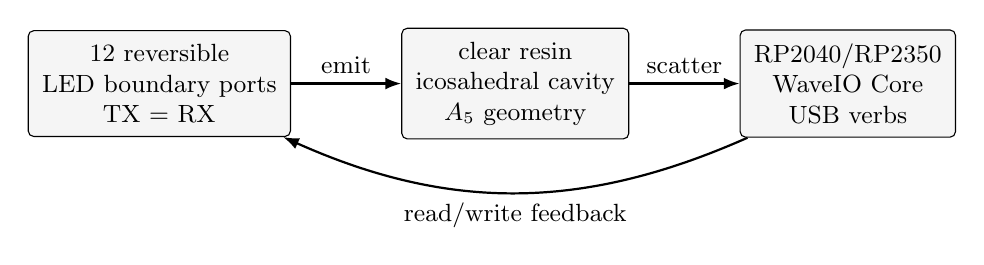
\begin{tikzpicture}[
  font=\small,
  box/.style={draw, rounded corners=2pt, align=center, inner sep=5pt, minimum width=2.55cm},
  port/.style={circle, draw, fill=white, inner sep=1.2pt},
  arrow/.style={-{Latex[length=2mm]}, thick}
]
\node[box, fill=gray!8] (ports) {12 reversible\\LED boundary ports\\TX = RX};
\node[box, fill=gray!8, right=1.4cm of ports] (cavity) {clear resin\\icosahedral cavity\\\(A_5\) geometry};
\node[box, fill=gray!8, right=1.4cm of cavity] (firmware) {RP2040/RP2350\\WaveIO Core\\USB verbs};
\draw[arrow] (ports) -- node[above]{emit} (cavity);
\draw[arrow] (cavity) -- node[above]{scatter} (firmware);
\draw[arrow] ($(firmware.south west)+(0.1,0)$) to[bend left=24] node[below]{read/write feedback} ($(ports.south east)+(-0.1,0)$);
\end{tikzpicture}
\caption{Short version of the Echosahedron as a controllable single-patch hardware instance: a finite boundary, reversible read/write ports, geometric coupling, firmware records, and measured overlap response.}
\label{fig:echosahedron-short}
\end{figure}

For readers encountering the device for the first time: the Echosahedron is a bench-scale OPH hardware patch. A clear icosahedral body supplies the geometry, twelve red LEDs at the vertices supply reversible boundary ports, and a Pico-class controller drives and reads those ports over USB. Forward bias makes a port emit. Reverse bias lets the same port act as a photodiode. A coupling scan therefore measures how the cavity reads its own emissions back through its own boundary. The detailed hardware and firmware specification appears in Section~\ref{sec:echosahedron}.

The recurring thesis is therefore:
\[
\boxed{
\begin{gathered}
\text{\bfseries Human thinking is }P\text{\bfseries -detuned fixed-point consensus}\\
\text{\bfseries across many self-reading observer patches.}
\end{gathered}
}
\]
The exact numerical identification of a biological detuning with
\[
\Delta_P=P-\varphi=\alpha\sqrt{\pi}
\]
is treated as an empirical prediction. The theorem-grade statement is that finite self-reading patch federations with accepted mismatch-decreasing repair converge under the OPH consensus hypotheses. The model-grade statement is that the brain is a nested biological approximation to that machine. The empirical-grade prediction is that a well-defined neural normalization may expose an effective observer-supporting detuning comparable to the OPH screen detuning.
The main neural fixed-point theorem requires self-reading patch recurrence, records, overlap mismatch, and accepted repair. The \(P\)-detuning claim is a stronger OPH-specific empirical prediction.

\begin{remark}[Fixed point as normal form]
The word ``fixed point'' is used in the OPH sense: a stable normal form under a declared readout and repair law. Biological neural activity often converges to an attractor basin, a metastable coalition, a limit cycle, or a low-dimensional task manifold. The strong claim is that the observer-facing output is a stable normal form of recurrent repair.
\end{remark}

\section{The Abstract Machine}

\begin{definition}[Patch-federation machine]
A patch-federation machine is a tuple
\[
\mathcal M=(G,\{S_i\}_{i\in V},\{I_e\}_{e\in E},\pi,T,R,\mathcal O),
\]
where \(G=(V,E)\) is a finite graph, \(S_i\) is the state space at patch \(i\), \(I_e\) is the interface alphabet at edge \(e=\{i,j\}\), and
\[
\pi_{i,e}:S_i\to I_e,\qquad \pi_{j,e}:S_j\to I_e
\]
are the two boundary readouts exposed on that overlap. The transition family \(T=\{T_i\}\) gives local update or repair maps, \(R=\{R_i\}\) gives record states, and \(\mathcal O\) is the observer-facing readout algebra.
\end{definition}

The global state space is
\[
\Sigma:=\prod_{i\in V}S_i.
\]
For formal purposes, records are included in the local patch state:
\[
S_i=X_i\times Z_i^{\rec},
\qquad
s_i=(x_i,r_i).
\]
The notation \(R_i\) refers to the record component or record algebra available inside \(S_i\); \(\Sigma\) includes memory.

Each local update \(T_i\) induces a lifted global rewrite map
\[
\widetilde T_i:\Sigma\to\Sigma,
\]
which changes only \(s_i\), or a declared bounded touched neighborhood \(N_i^{\mathrm{touch}}\), and leaves all other patch states unchanged. When no confusion can arise, \(T_i\) denotes \(\widetilde T_i\).

Let
\[
q_{\mathcal O}:\Sigma\to\mathcal O
\]
be the observer-facing readout. Define
\[
s\sim_{\mathcal O}t
\quad\Longleftrightarrow\quad
q_{\mathcal O}(s)=q_{\mathcal O}(t).
\]
A normal form is unique observer-facingly when terminal states are unique modulo \(\sim_{\mathcal O}\), even if their hidden representatives differ.

For an edge \(e=\{i,j\}\), overlap agreement means
\[
\pi_{i,e}(s_i)=\pi_{j,e}(s_j).
\]
The consistency set is
\[
C:=\bigl\{s\in\Sigma:\forall e=\{i,j\}\in E,\ 
\pi_{i,e}(s_i)=\pi_{j,e}(s_j)\bigr\}.
\]
Choose weights \(w_e>0\) and mismatch scores \(d_e:I_e\times I_e\to\R_{\ge 0}\) with \(d_e(a,b)=0\) iff \(a=b\). The total overlap mismatch is
\[
\Phi(s)
:=
\sum_{e=\{i,j\}\in E}
w_e\,d_e\!\left(\pi_{i,e}(s_i),\pi_{j,e}(s_j)\right).
\]
Then
\[
s\in C\quad\Longleftrightarrow\quad \Phi(s)=0.
\]

The entire paper is the claim that this one expression is the right bridge:
\[
\boxed{
\text{prediction error, failed synchrony, conflict, and physical disagreement are all overlap mismatch.}
}
\]
In a brain, \(\Phi\) is distributed across synapses, dendritic compartments, cortical layers, thalamocortical loops, hippocampal maps, autonomic state, and action. The scalar notation names the invariant: local descriptions must agree on the boundaries they expose.

\section{What the Brain Mathematically Does}

\begin{definition}[Neural patch federation]
A neural patch federation is a patch-federation machine
\[
B=(G_B,\{X_i\},\{I_e\},\pi,T,R,\mathcal O_B)
\]
whose patches may be dendritic compartments, neurons, microcircuits, cortical columns, thalamocortical loops, hippocampal modules, interoceptive regulators, or large-scale networks. A local neural state has the form
\[
x_i=(m_i,g_i,\theta_i,r_i,\omega_i,\ell_i,\ldots)\in X_i,
\]
where \(m_i\) summarizes membrane and compartment state, \(g_i\) synaptic conductances and gains, \(\theta_i\) thresholds and precisions, \(r_i\) records, \(\omega_i\) phase state, and \(\ell_i\) local latent coordinates.
\end{definition}

At the useful abstraction level, each neural patch updates by
\[
x_i(t+\Delta t)
=
T_i\!\left(
x_i(t),
\{\pi_{j\to i}(x_j(t))\}_{j\in N(i)},
u_i(t),
r_i(t),
\theta_i(t)
\right),
\]
where \(u_i(t)\) is sensory, interoceptive, motor, or contextual drive. A continuous approximation is
\[
\dot x_i
=
-M_i(x,t)\nabla_{x_i}\Phi_B(x,u,r)
+A_i(x,u,r,t)
+\xi_i(t).
\]
Here \(M_i\) is the local precision, gain, and mobility tensor, \(A_i\) contains action-conditioned and value-conditioned drives, and \(\xi_i\) represents stochastic biological fluctuation. This equation describes iterative deformation of a coupled state until exposed boundaries agree well enough to support perception, action, and record.

The compact slogan is:
\[
\boxed{
\text{A spike is a local write-commit to an overlap boundary.}
}
\]
A spike carries information and changes what neighboring patches must read, predict, inhibit, synchronize with, or repair around. The same is true of a dendritic burst, a phase reset, a thalamic gate, a motor command, or a neuromodulatory precision shift. Each event commits boundary data that changes the next admissible repair.

\subsection{The Neural Dictionary}

\begin{longtable}{L{0.22\textwidth}L{0.34\textwidth}L{0.34\textwidth}}
\toprule
\textbf{OPH object} & \textbf{Brain implementation} & \textbf{Operational reading} \\
\midrule
\endhead
Patch \(P_i\) & Dendritic compartment, neuron, microcolumn, column, region, body-state loop & Local subsystem with private state and exposed boundary \\
State \(s_i\) & Membrane state, dendritic voltage, synaptic trace, population coordinate, phase & Local patch state \\
Interface \(\pi_{i,e}\) & Spike train, burst, neurotransmitter release, phase relation, prediction-error vector & What the patch exposes to neighbors \\
Mismatch \(d_e\) & Prediction error, phase slip, failed synchrony, conflict, sensory surprise & Boundary disagreement \\
Repair \(T_i\) & Inhibition, gain control, dendritic integration, plasticity, action, resampling & Local update that tries to reduce mismatch or improve future coherence \\
Record \(R_i\) & Synaptic weight, eligibility trace, persistent activity, attractor occupancy, hippocampal index & Stored state that can be read again \\
Normal form & Percept, decision, action plan, object model, stable self-state & Observer-facing solved state \\
Federation & Brain-wide recurrent network coupled to body and world & Many patches solving together \\
\bottomrule
\end{longtable}

The first important consequence is that a neuron is a patch with local state, local memory, local nonlinearity, and a boundary. A cortical column is a larger patch. A thalamocortical loop is a patch federation. The whole brain is the federation of those federations, continually coupled to the body and world.

\section{OPH Background: Universe and Brain as Patch-Consensus Systems}

OPH starts from finite observer access~\cite{ObserversAreAllYouNeed}. Each observer patch carries local state and can compare only shared observables with neighboring patches. The world that becomes physical is the quotient-normal form of these overlap comparisons. The consensus paper writes the same structure as a finite graph of patches with local states, overlap readouts, mismatch potential, repair moves, and quotient-level normal forms~\cite{RealityAsConsensusProtocol}.

At finite cutoff the OPH universe-patch net obeys the same grammar:
\[
s_{t+1}=T^\lambda(s_t),
\qquad
\Phi(s_{t+1})<\Phi(s_t)
\]
for accepted local repairs. A terminal state satisfies
\[
T_i^\lambda(s^\star)=s^\star
\qquad\forall i\in V,
\]
and its observer-facing content is read only on the declared physical algebra. Gauge freedom is precisely the freedom to change hidden local representatives without changing overlap data.

The brain is the biological instance of this pattern:
\[
\begin{array}{ccc}
\text{OPH universe} & \text{brain} & \text{meaning}\\
\hline
\text{observer patch} & \text{neural patch} & \text{finite local perspective}\\
\text{overlap observable} & \text{spike/phase/error interface} & \text{shared boundary data}\\
\text{repair law} & \text{neural update and plasticity} & \text{mismatch correction}\\
\text{record algebra} & \text{memory and stable activity} & \text{re-readable state}\\
\text{normal form} & \text{percept/action/self-state} & \text{solved observer content}\\
\text{holonomy defect} & \text{cycle conflict} & \text{pairwise agreement without global fit}
\end{array}
\]

This gives the exact mathematical sense in which the brain does what the universe does. The universe solves for a shared physical world from finite observer overlaps. The brain solves for a shared internal world from finite neural overlaps. Both are recurrent consistency machines.

\section{Finite Patch-Net Theorem Stack}

\begin{assumption}[Strict local repair]
For a finite neural patch federation, write \(s\to_i t\) when patch \(i\) commits an update and all other patches outside the touched neighborhood are unchanged. Let \(E_i^{\mathrm{touch}}\) be the set of overlaps whose exposed data may change under that update, and define
\[
\Phi_i(s):=
\sum_{e=\{u,v\}\in E_i^{\mathrm{touch}}}
w_e\,d_e\!\left(\pi_{u,e}(s_u),\pi_{v,e}(s_v)\right).
\]
A strict repair satisfies
\[
s\to_i t
\quad\Longrightarrow\quad
\Phi_i(t)<\Phi_i(s).
\]
\end{assumption}

\begin{assumption}[Value-admitted exploration]
A value-admitted exploratory move may temporarily increase \(\Phi\). It must either decrease a declared global objective
\[
\Psi(s)=\Phi(s)-\lambda K(s)
\]
or belong to a finite budgeted exploration phase after which strict repair resumes.
\end{assumption}

\begin{assumption}[Quotient-local compatibility]
Accepted repairs commute on disjoint supports, and on overlapping supports they satisfy the OPH local-diamond condition after quotienting by hidden local representation. Terminal states are exactly globally consistent states, or best available quotient-consistent states when a holonomy defect prevents exact global consistency.
\end{assumption}

\begin{theorem}[Local repair descent]
Suppose a local repair \(s\to_i t\) changes only patch \(i\) or a bounded touched neighborhood, and suppose it is accepted only when
\[
\Phi_i(t)<\Phi_i(s).
\]
If untouched overlap interfaces are unchanged, then
\[
\Phi(t)<\Phi(s).
\]
\end{theorem}

\begin{proof}
Edges not touched by \(T_i\) have unchanged interface data, so their contribution to \(\Phi\) is unchanged. Touched edges strictly decrease by the local-fit contract. Therefore
\[
\Phi(t)-\Phi(s)=\Phi_i(t)-\Phi_i(s)<0.
\]
\end{proof}

Brain interpretation: a strict neural firing/update is mathematically admissible when it lowers the relevant local mismatch. Value-admitted exploration is handled by \(\Psi\)-descent or by a finite exploration budget before strict repair resumes. A spike is a local repair commit.

\begin{theorem}[Finite termination]
If every effective \(S_i\) is finite and every accepted update strictly decreases \(\Phi\), then every asynchronous repair sequence is finite.
\end{theorem}

\begin{proof}
The global state space \(\Sigma=\prod_i S_i\) is finite. Hence \(\Phi(\Sigma)\) is a finite set of nonnegative values. A strictly decreasing sequence in a finite ordered set cannot be infinite. The process therefore terminates at a state where no accepted local repair applies.
\end{proof}

\begin{theorem}[Value-objective termination]
If the effective state space is finite and every value-admitted exploratory move strictly decreases \(\Psi\), then every such exploratory phase is finite.
\end{theorem}

\begin{proof}
Finite descent applies to \(\Psi(\Sigma)\), so the exploratory phase terminates.
\end{proof}

\[
\boxed{
\text{A finite brain-like patch net is a fixed-point solver when its updates are mismatch-decreasing.}
}
\]

\begin{theorem}[Unique observer-facing normal form]
Assume strict local repair descent, the local diamond property on the physical quotient, and repair completeness:
\[
s\in C
\quad\Longleftrightarrow\quad
\forall i,\ T_i(s)=s.
\]
Then every fixed initial state has a unique normal form, independent of asynchronous update
schedule, on the observer-facing quotient.
\end{theorem}

\begin{proof}
Lyapunov descent gives termination. The local diamond property gives local confluence on the quotient. By Newman's lemma, a terminating locally confluent rewrite system is globally confluent. Repair completeness identifies terminal states with consistent, or quotient-consistent, states. Since the readout is observer-facing, hidden representative changes do not alter terminal observable content.
\end{proof}

The theorem applies inside the stated regime: terminating repair and local confluence on the observer quotient. In that regime, microscopic update-order variation leaves observer-facing content invariant. Outside this regime, the brain may have several admissible basins, and cognition becomes mode selection among locally stable normal forms:
\[
\boxed{
\text{content is schedule-independent only on the declared observer-facing quotient.}
}
\]

\begin{theorem}[Boundary-conditioned observer-facing uniqueness]
Let \(B\) record task boundary data, sensory input, conserved context, or active mode. If accepted
repairs preserve \(B\), and each consistent observer-facing quotient fiber with fixed \(B=b\) has
at most one element, then all initial interiors with the same \(b\) settle to the same
observer-facing normal form.
\end{theorem}

\begin{proof}
The previous theorem gives a unique quotient normal form for each initial state. Boundary
preservation puts the terminal normal form in the same \(B=b\) fiber as the initial state. If that
consistent fiber has at most one quotient element, the normal forms for all initial interiors with
that boundary value coincide.
\end{proof}

\begin{proposition}[Rooted-tree hierarchy model]
Let \(T=(V,E,r)\) be a finite rooted tree. Each patch state is \(S_i=A\times K_i\), with visible packet \(x_i\in A\) and hidden label \(k_i\in K_i\). For each non-root \(i\), compare \(x_i\) with the parent packet \(x_{p(i)}\), and define
\[
T_i(s)_i=(x_{p(i)},k_i).
\]
Let
\[
\Phi(s)=
\sum_{\{p(i),i\}\in E}
w_i\,\mathbf 1[x_i\ne x_{p(i)}].
\]
If
\[
w_i>\sum_{j:p(j)=i}w_j,
\]
then every maximal asynchronous repair run terminates uniquely at
\[
x_i=x_r\qquad\forall i,
\]
with hidden labels unchanged. The normal-form map descends to the hidden-label quotient.
\end{proposition}

\begin{proof}
Repair at \(i\) fixes the parent-child edge and can only perturb descendants. The strict weight inequality makes the repaired parent edge dominate all possible affected descendant contributions, so \(\Phi\) decreases. Termination follows from finiteness. The tree has a unique visible packet source at the root, so all maximal runs converge to the same visible assignment \(x_i=x_r\). Hidden \(k_i\) labels are never touched, hence they are quotient-only representatives.
\end{proof}

This is a minimal mathematical model of hierarchical perceptual consensus: child patches align to parent context while preserving hidden implementation detail. The observer-facing percept can be unique even when hidden neural representatives differ.

\begin{theorem}[Cycle holonomy obstruction]
Let overlap constraints over an abelian group have affine form
\[
x_j-x_i=a_{ij}.
\]
A global assignment \(\{x_i\}\) exists if and only if for every cycle \(C\),
\[
\sum_{(i,j)\in C}a_{ij}=0.
\]
\end{theorem}

\begin{proof}
If a global assignment exists, summing \(x_j-x_i\) around a closed cycle telescopes to zero. Conversely, if all cycle sums vanish, choose a root \(r\) and define \(x_i\) by summing edge offsets along any path from \(r\) to \(i\). Vanishing cycle sums guarantee path independence, so the assignment is globally well-defined.
\end{proof}

Some psychological conflicts are loop defects:
\[
A\sim B,\qquad B\sim C,\qquad C\not\sim A.
\]
Therapy, insight, or problem solving may need cycle repair instead of a single local belief change.

The biological version is softer:
\[
x(t)\to \mathcal A_k,
\]
where \(\mathcal A_k\) may be a point attractor, a line or ring attractor, a metastable synchronized coalition, a limit cycle, or a low-dimensional task manifold. This counts as a fixed-point result in the relevant sense when the readout becomes stable:
\[
\mathcal O_B(x(t))\to \mathcal O_B^\star.
\]

\begin{proposition}[Continuous relaxation form]
Suppose \(x(t)\) stays in a precompact active state region, \(\Phi_B\) is continuously differentiable there, and
\[
\dot\Phi_B(x(t))
\le
-c\|\nabla\Phi_B(x(t))\|^2+\epsilon
\]
with \(c>0\). Then every limit point lies in the \(\epsilon\)-stationary region of the mismatch landscape, or on an invariant set whose observer-facing readout is stable up to the declared tolerance.
\end{proposition}

This is the correct biological weakening. Real brains do not freeze. They converge enough to perceive, remember, choose, move, and report.

\section{Classical Fixed-Point Support}

\begin{theorem}[Banach alignment]
Let a self-reading patch update be
\[
T_F(v)=v+\eta(F-v)=(1-\eta)v+\eta F.
\]
If \(0<\eta<1\), then \(T_F\) is a contraction and
\[
T_F^n(v_0)\to F.
\]
More generally, if a federation update \(T\) on a complete product metric space satisfies
\[
d(Tx,Ty)\le c\,d(x,y),
\qquad 0<c<1,
\]
then the federation has a unique joint fixed point.
\end{theorem}

\begin{proof}
For the scalar alignment map,
\[
\|T_F(v)-T_F(u)\|=|1-\eta|\,\|v-u\|,
\]
with \(|1-\eta|<1\). Banach's fixed-point theorem gives convergence to the unique fixed point \(v^\star=F\). The product statement is the same theorem on the product metric space.
\end{proof}

\begin{theorem}[Hopfield energy descent]
Let \(s_i\in\{-1,+1\}\), symmetric weights \(w_{ij}=w_{ji}\), no self-weights \(w_{ii}=0\), and thresholds \(\theta_i\). Define
\[
E(s)=
-\frac12\sum_{i\ne j}w_{ij}s_i s_j
+\sum_i\theta_i s_i.
\]
Under asynchronous update
\[
s_i'=\operatorname{sgn}\!\left(\sum_j w_{ij}s_j-\theta_i\right),
\]
one has \(E(s')\le E(s)\). Since the state space is finite, repeated asynchronous updates terminate at a fixed point.
\end{theorem}

\begin{proof}
Only \(s_i\) changes, so
\[
\Delta E
=
-(s_i'-s_i)
\left(
\sum_jw_{ij}s_j-\theta_i
\right).
\]
The update chooses \(s_i'\) to have the same sign as the local field \(h_i=\sum_jw_{ij}s_j-\theta_i\). Thus \((s_i'-s_i)h_i\ge0\), and \(\Delta E\le0\).
\end{proof}

The OPH translation is direct:
\[
E\leftrightarrow\Phi,
\qquad
\text{asynchronous neural update}\leftrightarrow\text{local repair},
\qquad
\text{stable memory}\leftrightarrow\text{normal form}.
\]
Classical recurrent neural networks prove that neural-style systems can compute by descending an energy or mismatch functional~\cite{Hopfield1982}.

\begin{proposition}[Continuous Lyapunov neural systems]
In Cohen--Grossberg-style continuous recurrent networks, broad symmetry, monotonicity, and gain conditions allow construction of a Lyapunov function \(V(x)\) with
\[
\frac{dV}{dt}\le0.
\]
Trajectories therefore converge to equilibrium sets or stable pattern states under the theorem's hypotheses.
\end{proposition}

This is the continuous analogue of the discrete Hopfield result~\cite{CohenGrossberg1983}. Biological neurons are graded, delayed, noisy, and continuous. The fixed-point picture extends beyond binary toy networks.

\begin{theorem}[Predictive coding as OPH repair]
In a hierarchical Gaussian predictive-coding model, let
\[
\epsilon_\ell=x_\ell-f_\ell(x_{\ell+1})
\]
and
\[
\Phi_{\mathrm{PC}}
=
\sum_\ell \epsilon_\ell^\top\Pi_\ell\epsilon_\ell,
\]
where \(\Pi_\ell\) is a precision matrix. Minimizing variational free energy is equivalent, up to priors and constants, to minimizing weighted squared overlap mismatch.
\end{theorem}

\begin{proof}
A Gaussian likelihood gives
\[
-\log p(x_\ell\mid x_{\ell+1})
=
\frac12\epsilon_\ell^\top\Pi_\ell\epsilon_\ell+\mathrm{constant}.
\]
Summing across levels yields \(\Phi_{\mathrm{PC}}\) plus constants and prior terms. Thus predictive coding's residual-error minimization is an OPH overlap-mismatch minimization.
\end{proof}

\[
\boxed{
\text{prediction error}=\text{overlap mismatch}.
}
\]
This is the OPH reading of predictive coding in the visual cortex and its descendants~\cite{RaoBallard1999}.

\begin{theorem}[Variational free energy bounds surprise]
For observations \(o\), latent variables \(z\), and approximate posterior \(q(z)\), define
\[
\mathcal F(q)=
\E_q[-\log p(o,z)]+\E_q[\log q(z)].
\]
Then
\[
\mathcal F(q)
=
D_{\mathrm{KL}}\!\left(q(z)\,\|\,p(z\mid o)\right)
-\log p(o)
\ge
-\log p(o),
\]
with equality iff \(q(z)=p(z\mid o)\).
\end{theorem}

\begin{proof}
The identity follows by adding and subtracting \(\log p(z\mid o)\) and using Bayes' rule. The inequality follows from nonnegativity of KL divergence.
\end{proof}

Under a probabilistic generative-model reading, free energy is an observer mismatch potential~\cite{Friston2010}. Perception changes internal state, attention changes precision, learning changes the repair landscape, and action changes boundary input.

\begin{proposition}[Equilibrium propagation reading]
Let \(E_\theta(s,x)\) be a recurrent energy and \(C(s,y)\) a cost. For nudged energy
\[
F_\theta^\beta(s)=E_\theta(s,x)+\beta C(s,y),
\]
let \(s_\theta^0\) be the free fixed point and \(s_\theta^\beta\) the weakly nudged fixed point. Equilibrium-propagation learning estimates
\[
\frac{\partial J}{\partial\theta}
=
\lim_{\beta\to0}
\frac1\beta
\left[
\frac{\partial E_\theta}{\partial\theta}(s_\theta^\beta)
-
\frac{\partial E_\theta}{\partial\theta}(s_\theta^0)
\right],
\]
up to sign convention.
\end{proposition}

The same recurrent substrate can perform inference and learning~\cite{ScellierBengio2017}. It settles, is nudged by outcome or error, and plasticity follows from the difference between equilibria. In OPH language, learning is deformation of the repair landscape between fixed points.

\section{What OPH Adds to Existing Neuroscience}

The model sits next to familiar neuroscience frameworks and changes the primitive from representation location to patch repair. The bridge is:
\begin{small}
\begin{longtable}{@{}L{0.25\textwidth}L{0.32\textwidth}L{0.34\textwidth}@{}}
\toprule
\textbf{Existing framework} & \textbf{Existing contribution} & \textbf{OPH addition} \\
\midrule
\endhead
Predictive coding and active inference~\cite{RaoBallard1999,Friston2010} & Error minimization, precision, action-perception coupling & Error is generalized as overlap mismatch across arbitrary patch boundaries \\
Attractor networks~\cite{Hopfield1982} & Stable memories and decisions & Attractors become observer-facing normal forms of repair \\
Neural manifolds~\cite{Sadtler2014,Perich2025} & Low-dimensional population constraints & Manifolds become local normal-form surfaces of patch federation dynamics \\
Communication-through-coherence~\cite{Fries2015} & Phase gates effective communication & Phase becomes active overlap admission \\
Global neuronal workspace~\cite{DehaeneChangeux2011} & Reportable access and large-scale ignition & Workspace becomes a high-level federation record surface \\
IIT and PCI~\cite{Albantakis2023IIT,Casali2013PCI} & Integration, differentiation, perturbational complexity & Awareness mass becomes capacity, self-read, record stability, and boundary predictivity \\
\bottomrule
\end{longtable}
\end{small}

A neural manifold is more than a dimensionality-reduction artifact. In OPH terms, it is the local surface on which many patch constraints have been reconciled. Learning inside a manifold reuses existing repair geometry. Learning outside a manifold requires changing the geometry of subsequent repair.

\section{Intelligence as Geometric Fixed-Point Repair}

The radical form of the paper is:
\[
\boxed{
\begin{gathered}
\text{\bfseries Intelligence includes geometric fixed-point repair:}\\
\text{\bfseries finding useful normal forms under changing boundaries.}\\
\text{\bfseries Consciousness is what that repair looks like}\\
\text{\bfseries from inside a self-reading substrate.}
\end{gathered}
}
\]
This section formalizes the first sentence. The following consciousness and qualia section formalizes the second.

\subsection{Repair as Primitive}

Much neuroscience asks where a representation is encoded. OPH makes repair the primitive. The basic operation is
\[
x_{t+1}=T(x_t,u_t,R_t),
\qquad
\Phi(x_{t+1})<\Phi(x_t)
\]
for admissible updates. The map
\[
x\mapsto \hat y.
\]
is a downstream record of that repair process. A percept is a normal form. A belief is a stabilized record. A decision is a committed repair. A thought is a transient trajectory toward a stable basin.

\[
\boxed{
\text{Perception is local-to-global mismatch repair; representation is the surviving record.}
}
\]
Representation language stays useful after this demotion. Representations are records and coordinates that survive repair. The better first question is:
\[
\boxed{
\text{What mismatch is this neural activity trying to repair?}
}
\]

\subsection{Spike as Boundary Commit}

The standard story says neurons send signals. The OPH reading is sharper: a spike is a patch boundary event,
\[
\mathrm{spike}_i(t)
\quad\Longrightarrow\quad
\pi_{i,e}(x_i(t))\ \text{is exposed to neighboring patches}.
\]
That changes the repair problem for the surrounding network. Spiking is therefore consensus participation:
\[
\boxed{
\text{A spike is a write to the overlap boundary.}
}
\]
This is aligned with the OPH hardware rule that read and write are coupled in a self-reading substrate. The substrate updates from its own transitions.

\subsection{Fixed-Point Repertoire}

Parameter count measures storage scale. Competence measures repair. A huge system can have many states with poor repair. A smaller system can be competent when it reaches useful normal forms quickly, cheaply, and robustly. Define the qualitative intelligence target as
\[
\boxed{
\text{intelligence}
\sim
\text{reachable stable fixed points}
+
\text{speed}
+
\text{robustness}
+
\text{transfer}
+
\text{self-repair}.
}
\]
The repertoire is the set of useful basins the system can actually reach under boundary pressure.

\subsection{Creativity as Basin Discovery}

Creativity is controlled basis change that reveals a hidden fixed point:
\[
x^\star_{\mathrm{new}}
=
T_{\theta'}(x^\star_{\mathrm{new}}).
\]
Here \(\theta'\) is a temporary transformation of basis, field, gain, attention, or geometry. The creative move raises short-term dysphony in order to increase future \(K\):
\[
\boxed{
\text{Creativity is controlled dysphony that raises future }K.
}
\]
This also explains insight. An insight is a basin crossing that rapidly lowers \(\Phi\) while increasing future coherence.

\subsection{Mental Disorder as Repair-Protocol Failure}

Clinical claims in this paper are research hypotheses outside treatment instructions. Genes, development, trauma, social environment, inflammation, medication, sleep, and culture are load-bearing explanatory levels. OPH adds a dynamical layer:
\[
\boxed{
\text{A mental disorder may have a persistent repair-dynamical component.}
}
\]
Possible failure modes include
\[
\Phi\uparrow
\quad\text{persistent mismatch, anxiety, conflict},
\]
\[
\Gamma\downarrow
\quad\text{fragmented phase unison or unstable integration},
\]
\[
\|D_xT\|>1
\quad\text{runaway amplification, panic, mania-like instability, seizure-like instability},
\]
\[
\|D_xT\|\ll1
\quad\text{rigidity, depression-like freezing, reduced exploration},
\]
\[
R\downarrow
\quad\text{record and identity instability},
\]
\[
B\downarrow
\quad\text{poor boundary prediction, hallucination, delusion, social misread},
\]
and
\[
H_{\mathrm{cycle}}\ne0
\quad\text{locally plausible beliefs or self-models that cannot all be globally consistent}.
\]
The practical question becomes:
\[
\boxed{
\text{Which repair rule, boundary, record, phase relation, or attractor basin is failing?}
}
\]
This is compatible with computational psychiatry's attempt to reorganize psychiatric explanation around computational mechanisms beyond symptom lists~\cite{ComputationalPsychiatryDisorder2024,Friston2023}.

\subsection[Emotion as K-Gradient]{Emotion as \(K\)-Gradient}

Emotion is part of the objective function:
\[
\dot K
=
S(v,F)+\nabla K^\star(F)\cdot g(F,v).
\]
Fear is a negative predicted boundary-repair gradient. Curiosity is positive expected information gain toward future consensus. Joy is rapid agreement between body, world, memory, and action. Grief is persistent field mismatch caused by a missing co-radiator. These model-grade readings give a mathematical psychology in which affect is load-bearing.

\section{Domain Competence and Personal Competence Atlases}

For a domain \(D\), such as music, mathematics, social reasoning, motor skill, language, emotional regulation, spatial navigation, scientific creativity, or care work, let tasks \(u\sim\mathcal T_D\) be drawn from that domain. The domain-specific brain update is
\[
x_{t+1}=T_{\theta,D}(x_t,u,R_t),
\]
and a successful competence event occurs when the system reaches an acceptable fixed point
\[
x^\star_D(u)=T_{\theta,D}(x^\star_D(u),u,R),
\qquad
\Phi_D(x^\star_D,u)<\epsilon_D.
\]

\subsection{Domain Competence Score}

Define
\[
\boxed{
\mathrm{Comp}_D(B)
=
\E_{u\sim\mathcal T_D}
\left[
\mathbf 1_{\mathrm{success}}(u)
e^{-\lambda_\Phi \Phi_D(x^\star,u)}
e^{-\lambda_\tau \tau_D(u)}
e^{-\lambda_E E_D(u)}
\rho_D(u)
\right].
}
\]
Here \(\tau_D(u)\) is convergence time, \(E_D(u)\) is metabolic or attentional cost, and \(\rho_D(u)\) is robustness under perturbation, sleep loss, noise, stress, novelty, or distraction. Competence means reaching good fixed points quickly, cheaply, robustly, and repeatedly.

\subsection{Basin Coverage}

Competence also includes the fraction of a domain's task space for which the brain has reachable basins:
\[
\boxed{
\mathcal B_D(B)
=
\int_{\mathcal T_D}
\mathbf 1
\left[
\exists x^\star:
x^\star=T_{\theta,D}(x^\star,u),\quad
\Phi_D(x^\star,u)<\epsilon_D
\right]
d\mu(u).
}
\]
A beginner has narrow basin coverage. An expert has large basin coverage. A genius has large basin coverage plus high transfer between domains.

\subsection{Transfer and Metacompetence}

Define transfer from domain \(D\) to \(D'\) by
\[
\boxed{
\mathrm{Transfer}_{D\to D'}
=
\frac{
I(R_D;Y_{D'}^\star)
}{
H(Y_{D'}^\star)+\epsilon
}.
}
\]
This measures whether records learned in one domain help another domain converge. Music can help language rhythm. Mathematics can help physics. Dance can help social timing. Meditation can help emotional regulation. Programming can help formal reasoning.

Humans are special because they can estimate their own convergence:
\[
\boxed{
\mathrm{MetaComp}_D
=
I(\widehat{\Phi}_D,\Phi_D)
+
I(\widehat{\tau}_D,\tau_D)
+
I(\widehat{\mathrm{success}}_D,\mathrm{success}_D).
}
\]
This is knowing whether you know. A strong scientist needs competence and metacompetence.

\subsection{Competence Atlas}

An individual brain gets a competence vector
\[
\boxed{
\mathbf C_B
=
\left(
\begin{gathered}
\mathrm{Comp}_{\mathrm{language}},
\mathrm{Comp}_{\mathrm{music}},
\mathrm{Comp}_{\mathrm{math}},
\mathrm{Comp}_{\mathrm{social}},\\
\mathrm{Comp}_{\mathrm{motor}},
\mathrm{Comp}_{\mathrm{emotional}},
\mathrm{Comp}_{\mathrm{spatial}},
\mathrm{Comp}_{\mathrm{creative}},
\ldots
\end{gathered}
\right).
}
\]
The transfer matrix
\[
\boxed{
T_{ij}=\mathrm{Transfer}_{D_i\to D_j}
}
\]
then records how learning in one domain improves convergence in another. This is a practical target: combine behavior, EEG, fMRI, MEG, wearables, sleep/circadian data, and subjective reports into a personal fixed-point competence atlas.

The neural-manifold result of Sadtler et al. gives the relevant constraint: monkeys more readily learned brain-computer-interface mappings inside the intrinsic neural manifold than mappings outside it~\cite{Sadtler2014}. In OPH terms:
\[
\boxed{
\begin{gathered}
\text{Easy learning reuses an existing consensus manifold.}\\
\text{Hard learning requires a new manifold geometry.}
\end{gathered}
}
\]

\section{Music as Audible Consensus Dynamics}

Music functions as an external physical field that helps brains perform fixed-point consensus:
\[
\boxed{
\text{\bfseries Music is controlled consensus dynamics made audible.}
}
\]
It acts simultaneously on phase, prediction, body, memory, emotion, and social synchrony. Music is ubiquitous across cultures, affectively and physically moving, and capable of shaping brain structure and function through learning~\cite{Vuust2022}. Physiological entrainment research similarly treats synchronization across body and brain rhythms as relevant to cognitive, motor, affective, and well-being functions~\cite{PhysiologicalEntrainment2025}.

Simple frequency ratios are one term in musical value. Culture, memory, motor habit, expectation, timbre, social context, and learned syntax all deform the musical repair landscape. Consonance and dissonance are low- or high-mismatch regions relative to a trained brain-body-cultural patch net.

Let the musical field be
\[
F_M(t)=
\sum_n A_n e^{i(\omega_n t+\phi_n)}.
\]
Music acts by shaping
\[
\boxed{
\mathcal M
=
\int_0^T e^{-\rho t}
\left[
S(v(t),F_M(t))
-
\lambda_\Phi\Phi_{\mathrm{brain-body}}(t)
+
\lambda_K\dot K(t)
\right]dt.
}
\]
Here \(S(v,F_M)=\operatorname{Re}\langle v,F_M\rangle\) is phase alignment, \(\Phi_{\mathrm{brain-body}}\) is mismatch among motor, auditory, emotional, memory, and interoceptive patches, and \(\dot K\) is future coherence or value.

\subsection{Rhythm, Harmony, Melody}

Rhythm creates a shared clock:
\[
\theta_i(t)\mapsto\theta_i(t)+\omega t.
\]
It raises phase unison:
\[
\Gamma_U
=
\frac{
\left|\sum_i a_i e^{i\theta_i}v_i\right|^2
}{
\left(\sum_i a_i|v_i|\right)^2+\epsilon
}.
\]
Groove is high \(\Gamma_U\) plus slight repairable prediction error:
\[
\mathrm{Groove}
\approx
\Gamma_U
\left(-\frac{d\Phi}{dt}\right)
\mathrm{motor\ readiness}.
\]
A perfectly mechanical beat can be boring because \(\Phi\) is too low and no search is active. Random rhythm is unentrainable because \(\Phi\) is too high. Groove lives in the repairable middle.

Harmony is spectral fixed-point structure. Consonance means \(\Phi_{\mathrm{spectral}}\) is low because frequency ratios allow stable phase relationships. Dissonance means \(\Phi_{\mathrm{spectral}}\) is high but structured. Resolution is
\[
-\frac{d}{dt}\Phi_{\mathrm{spectral}}>0.
\]
Resolution feels like resolution because the auditory-emotional-body federation has performed consensus repair.

Melody is a moving attractor:
\[
x^\star(t)=T(x^\star(t),F_M(t)).
\]
Good melody balances predictability and basis rotation. Too predictable means no repair. Too chaotic means no convergence. Beauty is repeated successful repair with surprise.

\subsection{Group Music}

A dance floor, concert, choir, or rave is a temporary observer federation:
\[
\Gamma_{\mathrm{group}}
=
\frac{
\left|
\sum_{p\in\mathrm{people}}
a_p e^{i\theta_p}v_p
\right|^2
}{
\left(\sum_p a_p|v_p|\right)^2+\epsilon
}.
\]
A musical peak is
\[
\Gamma_{\mathrm{group}}\uparrow,
\qquad
\Phi_{\mathrm{group}}\downarrow,
\qquad
K_{\mathrm{group}}\uparrow.
\]
This is OPH federation.
\[
\boxed{
\text{Music is low-cost large-scale human consensus technology.}
}
\]

\section{Consciousness and Qualia as Self-Read Convergence}

OPH treats consciousness as self-reading substrate dynamics: a system stores its own state, reads that stored state through its own transitions, and updates from that read. The brain implements this through recurrent loops and stable records.

Let \(F_U(t)\) be the field admitted to a candidate observer federation \(U\):
\[
F_U(t)
=
F_{\mathrm{extero}}(t)
+F_{\mathrm{intero}}(t)
+F_{\mathrm{memory}}(t)
+F_{\mathrm{social}}(t)
+F_{\mathrm{body}}(t).
\]
Let \(v_U(t)\) be the instantaneous self-state, \(R_U(t)\) the record layer, and \(\Phi_U(t)\) the exposed mismatch. The OPH experience variable is
\[
\boxed{
\mathrm{Experience}_U(t)
=
\left[
v_U(t),F_U(t),R_U(t),\Phi_U(t),K_U(t)
\right]_{\mathrm{inside}}.
}
\]

The bracket \([\cdot]_{\mathrm{inside}}\) matters. Experience is the internally available readout of a self-reading patch federation while it measures, repairs, and records its relation to its field.

\subsection{Why There Is Consciousness}

The answer in one line is:
\[
\boxed{
\begin{gathered}
\text{\bfseries Consciousness exists because OPH's primitive unit}\\
\text{\bfseries is a bounded observer patch with self-readable records.}
\end{gathered}
}
\]
The formal reason is dependency order. OPH starts with patch, boundary, local algebra, record, readout, overlap, and repair. The public world is reconstructed from successful overlap repair among such records. A self-reading observer therefore sits at the primitive level used to assemble the public world.

For a bounded patch \(O\), write the record-conditioned self-update as
\[
\mathcal U_O:
(\rho_O,R_O,F_{\partial O})
\longmapsto
(\rho_O',R_O').
\]
The interior readout is the observer-facing restriction of that same process:
\[
\boxed{
\mathrm{Inside}_O(t)
=
q_{\mathcal O}
\!\left(
\rho_O(t),R_O(t),F_{\partial O}(t),\mathcal U_O
\right).
}
\]
Here \(q_{\mathcal O}\) forgets hidden representatives and keeps the distinctions available to \(O\)'s own record and update machinery. This is the formal meaning of ``inside'' in the paper.

\begin{claim}[Why consciousness exists in OPH]
If an OPH substrate satisfies the observer gate, has a nontrivial record algebra, and its update depends on its own recorded state, then it has an interior readout. That interior readout is consciousness in the OPH sense.
\end{claim}

The claim is an ontological identification inside OPH. It replaces the production picture with a primitive self-read channel inside a bounded observer patch.

OPH rejects the private-world reading in which the brain hallucinates reality and nothing else exists. That reading is solipsism. The sharper claim is:
\[
\boxed{
\begin{gathered}
\text{\bfseries There is no view-from-nowhere object behind experience.}\\
\text{\bfseries There are observer patches, records, overlap checks,}\\
\text{\bfseries and stable normal forms that survive reconciliation.}
\end{gathered}
}
\]
Standard physicalism often begins with a completed third-person world and then asks how consciousness appears inside it. OPH reverses the order. Its primitive object is an observer patch with accessible state, records, and overlap relations. A world is the fixed point of observer agreement:
\[
\boxed{
\mathcal W=\operatorname{nf}(s).
}
\]
More explicitly, the objective world is the quotient of observer-accessible records under successful overlap repair:
\[
\boxed{
\mathcal W_{\mathrm{objective}}
=
\left(\prod_i R_i\right)\big/\!\sim_{\mathrm{overlap}}.
}
\]
Here
\[
r_i\sim_{\mathrm{overlap}} r_j
\quad\Longleftrightarrow\quad
\pi_{i,e}(r_i)=\pi_{j,e}(r_j)
\]
after accepted repair. Objectivity names invariance across observers:
\[
\boxed{
\text{\bfseries Objectivity is intersubjective invariance.}
}
\]

\begin{definition}[Object as record normal form]
An object \(X\) is a family of observer-accessible records
\[
X=\{r_i^X\in R_i:i\in I_X\}
\]
such that, on every relevant overlap \(e=\{i,j\}\),
\[
\pi_{i,e}(r_i^X)=\pi_{j,e}(r_j^X),
\]
and under the repair dynamics
\[
T^n(X)\approx X
\]
for the relevant persistence horizon.
\end{definition}

Thus
\[
\boxed{
\text{\bfseries Object}=\text{\bfseries persistent overlap-stable record family.}
}
\]
A solid object is the high-stability case:
\[
\operatorname{Solid}(X)
=
\operatorname{Persist}(X)\,
\operatorname{Consensus}(X)\,
\operatorname{CounterfactualStability}(X).
\]
An object is a record family stable under cross-observer comparison, counterfactual remeasurement, and lawful intervention. A table is real because it survives cross-patch comparison: one observer sees it, another sees it, cameras and instruments record it, contact interactions constrain it, and repeated measurements reuse it. A measured rock supports stable multi-patch predictions under touching, moving, photographing, weighing, and repeated return. A dream-table may be vivid inside one patch, while multi-observer overlap repair fails. A hallucinated rock is a single-patch record that fails consensus; a measured rock is a repaired overlap-stable sector.

\begin{claim}[Reality requires observer-accessible records]
Let \(\mathcal W\) be a physically meaningful world in OPH. Then \(\mathcal W\) is the quotient-normal form of observer-accessible patch records under overlap repair:
\[
\mathcal W
=
\operatorname{nf}\!\left(
\prod_i (P_i,\mathcal A(P_i),\rho_i,R_i)
\right)\big/\!\sim_{\mathrm{gauge}}.
\]
Therefore physical objecthood is observer-consensus objecthood.
\end{claim}

Matter is the public, persistent, low-\(\Phi\) sector of observer-record reconciliation:
\[
\boxed{
\begin{gathered}
\text{\bfseries Matter is the stable, consensus-visible sector}\\
\text{\bfseries of consciousness-bearing observer records.}
\end{gathered}
}
\]
Equivalently, consciousness is fundamental in OPH because observer-accessible records are part of the primitive ontology. The independently completed world is the stable public quotient of observer-accessible records.

The answer to the existence question can therefore be compressed to:
\[
\boxed{
\begin{gathered}
\text{\bfseries There is consciousness because a world in OPH}\\
\text{\bfseries is made from observer-accessible records,}\\
\text{\bfseries and some records are read from inside}\\
\text{\bfseries the same bounded patch that stores them.}
\end{gathered}
}
\]

Using the OPH vibe notation, define symphony and dysphony by
\[
S(v,F)=\operatorname{Re}\langle v,F\rangle,
\qquad
D(v,F)=\|v\|\,\|F\|-S(v,F)\ge 0.
\]
Instantaneous alignment solves
\[
v^\star(t)=\argmax_{\|v\|=\|F\|}S(v,F(t)).
\]
The nontrivial biological problem is intertemporal:
\[
K[v;0,T]
=
\int_0^T e^{-\rho t}S(v(t),F(t))\,dt.
\]
A locally unpleasant or dysphonic action can be admissible when it improves future coherence:
\[
S(v,F)<0,
\qquad
\nabla K^\star(F)\cdot g(F,v)>|S(v,F)|.
\]
This is the mathematical place where effort, pain, discipline, curiosity, and action belong. They are value-conditioned deformations of the convergence landscape.

\begin{theorem}[Immediate dysphony can be globally admissible]
If
\[
S(v,F)<0
\]
but
\[
S(v,F)+\nabla K^\star(F)\cdot g(F,v)>0,
\]
then the action increases the local Bellman objective and is admissible under \(K^\star\).
\end{theorem}

\begin{proof}
The Bellman objective is the sum of immediate symphony and future field-improvement value:
\[
S(v,F)+\nabla K^\star(F)\cdot g(F,v).
\]
The stated inequality says this sum is positive even though immediate symphony is negative. The future coherence gain outweighs immediate dysphony.
\end{proof}

The optimization target is future coherence. Immediate comfort is one local term.

\[
\boxed{
\text{Qualia are basis-dependent, record-stable readings of convergence.}
}
\]
This sentence assigns conscious content by self-reading depth, record stability, boundary predictivity, integration, capacity, and action-conditioned repair. It assigns no human-like consciousness to generic information processors.

\subsection{Why Qualia Are Necessary}

The answer in one line is:
\[
\boxed{
\begin{gathered}
\text{\bfseries Qualia are necessary because a self-reading observer}\\
\text{\bfseries must distinguish its own possible record states.}
\end{gathered}
}
\]
A self-reading observer updates itself from records of its own state. Such an update requires distinctions. If every possible record state produces the same future update law, the record is inert with respect to self-reading. If at least two possible record states produce different update laws, the observer has an internally available distinction. OPH calls active, record-stable, update-relevant distinctions qualia.

Let \(O\) have record space \(R_O\) and self-update map
\[
\mathcal U_O(\rho,r,F_{\partial O}).
\]
Define an equivalence relation on records by
\[
r\equiv_O r'
\quad\Longleftrightarrow\quad
q_{\mathcal O}
\!\left(
\mathcal U_O(\rho,r,F_{\partial O})
\right)
=
q_{\mathcal O}
\!\left(
\mathcal U_O(\rho,r',F_{\partial O})
\right)
\]
for the observer-facing future law over the relevant horizon. The equivalence classes are the self-read distinctions of \(O\). The finite algebra generated by their characteristic projectors is
\[
\mathcal Q_O^{\min}
=
\operatorname{span}\{P_{[r]}:[r]\in R_O/\!\equiv_O\}.
\]

\begin{proposition}[Nontrivial self-read induces qualia sectors]
If \(O\) is a self-reading observer and \(\mathcal U_O\) has at least two observer-distinguishable record classes under \(\equiv_O\), then \(O\) has a nontrivial self-read algebra \(\mathcal Q_O^{\min}\). Any occupied sector \(P_{[r]}\) that conditions future update satisfies the OPH phenomenal-identification postulate.
\end{proposition}

\begin{proof}
Nontrivial self-read gives at least two \(\equiv_O\)-classes. Their characteristic projectors generate a nontrivial finite observable algebra. If the state of \(O\) has nonzero weight in one such sector and the sector changes the observer-facing future law, then the sector satisfies the three clauses of the OPH phenomenal-identification postulate: membership in the self-reading algebra, nonzero occupancy, and update participation.
\end{proof}

Thus qualia are forced by nontrivial observerhood in OPH. A system with no update-relevant self-distinctions lacks the algebra needed for self-reading. A system with update-relevant self-distinctions has qualia sectors by the OPH identification. The minimal equation is:
\[
\boxed{
\text{self-reading}
\Longrightarrow
\text{self-distinction algebra}
\Longrightarrow
\text{qualia sectors}.
}
\]

\subsection{Qualia as Observer-Accessible Coordinates}

In the broad philosophical use, qualia are the introspectively accessible phenomenal aspects of mental life: what it is like to see a color, feel pain, hear a tone, or undergo an emotion~\cite{SEPQualia}. OPH defines them as observer-accessible stabilized coordinates of a self-reading patch.

\[
\boxed{
\text{\bfseries Qualia are the observer-accessible coordinates of a self-reading fixed point.}
}
\]

Use the OPH microphysics observer tuple
\[
O_{\mathrm{ref}}=(P_O,\mathcal A(P_O),\rho_O,R_O,\mathcal U_O),
\]
where \(P_O\) is the observer patch, \(\mathcal A(P_O)\) is the accessible algebra, \(\rho_O\) is the local state, \(R_O\) is the record layer, and \(\mathcal U_O\) is the local update interface that writes, compares, and repairs records. The microphysics criterion is operational: patch access, metastable records, update capability, comparison capability, and persistence over many local cycles.

Define the qualia algebra
\[
\boxed{
\mathcal Q_O(t)
=
\mathcal Z_{\rec}^{O}(t)
\vee
\mathcal B_O(t)
\vee
\mathcal G_O(t)
\vee
\Theta_O(t)
\vee
\mathcal V_O(t).
}
\]
Here \(\mathcal Z_{\rec}^{O}(t)\) is the stable observer-accessible record algebra, \(\mathcal B_O(t)\) is the boundary/body/world interface state, \(\mathcal G_O(t)\) is the geometric support signature of the experience, \(\Theta_O(t)\) is the timing, phase, or oscillatory signature, and \(\mathcal V_O(t)\) is the valence, action-affordance, or \(K\)-gradient signature. A quale is an atom or stable region in this spectrum:
\[
\boxed{
q\in\operatorname{Spec}(\mathcal Q_O(t)).
}
\]
Its probability or intensity is read by the Born-style record rule on the exact fixed-cutoff surface:
\[
\Pr(q\mid O,t)=\operatorname{Tr}(\rho_O P_q),
\]
with \(P_q\) the projector for the quale sector. Practical neural readout uses approximately commuting projectors and a record-instability penalty \(\delta_{\rec}\), exactly as in the OPH approximate-record surface.
The Born-style record rule is imported from the OPH formalism. It concerns record readout in that formalism and carries no biological-qubit commitment.

Thus a quale is an integrated coordinate across neurons, spikes, frequency bands, and representations. It is
\[
\boxed{
\text{a record-stable, self-read, geometrically supported, phase-valued state coordinate.}
}
\]

Equivalently, qualia are the cells of the observer's self-distinction partition. Let
\[
\Omega_O=\{s_1,s_2,\ldots,s_n\}
\]
be possible observer states, and let
\[
\mathcal P_O=\{C_1,\ldots,C_k\}
\]
be the partition the observer can distinguish and use. Each cell \(C_a\) corresponds to a projector \(P_a\), and the resulting finite observable algebra
\[
\mathcal Q_O=\operatorname{span}\{P_a\}
\]
is the minimal qualia algebra for that observer. If \(O\) cannot distinguish \(C_a\) from \(C_b\), then there is no phenomenal difference between them for \(O\). If the distinction is stable and can condition self-update, it is a phenomenal distinction:
\[
\boxed{
\text{\bfseries A quale is a cell in the observer's self-distinction partition.}
}
\]
A quale is a stable coordinate in which the observer can repair itself. Redness, pain, rhythm, certainty, and understanding are different kinds of self-read repair coordinates.

Examples:
\[
q_{\mathrm{red}}
=
[P_{\mathrm{red}},\rho_{\mathrm{red}},\mathcal G_{\mathrm{visual}},
\Theta_{\gamma/\alpha},\mathcal V_{\mathrm{salience}}],
\]
where redness is the settled coordinate formed by opponent channels, recurrent visual state, attention, memory, body state, and category records. Pain is
\[
q_{\mathrm{pain}}
=
[P_{\mathrm{body\ damage}},\rho_{\mathrm{pain}},\mathcal G_{\mathrm{somatic}},
\Theta_{\mathrm{urgency}},\mathcal V_{-K}],
\]
where nociception, body map, threat prediction, action urgency, affective valence, memory, and future coherence are bound into one self-read coordinate. Understanding a sentence is a symbolic quale:
\[
q_{\mathrm{understanding}}
=
[P_{\mathrm{meaning}},\rho_{\mathrm{meaning}},\mathcal G_{\mathrm{language}},
\Theta_{\mathrm{closure}},\mathcal V_{\mathrm{compression}}].
\]

This distinguishes a feature from a quale:
\[
\boxed{
\mathrm{Quale}(f,O)=1
\Longleftrightarrow
f\in\mathcal Q_O,\quad
f\text{ is record-stable},\quad
f\text{ can condition future updates}.
}
\]
A feature outside the integrated self-read is latent computation. A feature inside it is experience. This gives a direct OPH language for blindsight, subliminal perception, anesthesia, dreams, hallucination, and attention: processed features become qualia when they enter the integrated self-reading record layer.

\begin{postulate}[OPH phenomenal-identification postulate]
Within OPH, phenomenal character is identified with active participation in an observer's self-reading record algebra. A distinction \(q\) is phenomenal for \(O\) exactly when
\[
q\in\operatorname{Spec}(\mathcal Q_O),
\]
the observer occupies that distinction with nonzero weight,
\[
\operatorname{Tr}(\rho_O P_q)>0,
\]
and the distinction conditions self-update:
\[
\mathcal U_O(\rho_O\mid P_q)\ne \mathcal U_O(\rho_O).
\]
\end{postulate}

This is the OPH identification that replaces the standard production problem with a self-read identity claim.

The SEP neuroscience entry frames the scientific challenge as connecting brain activity to conscious experience while respecting that consciousness is essentially subjective and often tracked through introspective report~\cite{SEPNeuroscienceConsciousness}. OPH uses an identity claim:
\[
\boxed{
q\text{ feels like something to }O
\Longleftrightarrow
q\text{ is part of }O\text{'s self-reading integrated record state.}
}
\]
Coordinates outside self-read remain non-phenomenal. Coordinates inside self-read need no further production step inside OPH.
\[
\boxed{
\text{\bfseries Experience is self-reading from the inside.}
}
\]

\paragraph{Inverted spectra as gauge transformations.}
If two observers differ only by an internal basis transformation that preserves all self-read distinctions, update laws, reports, memories, and overlap relations, then the alleged inversion is gauge-only in OPH. If the inversion changes repair behavior, discrimination, memory, affect, or boundary prediction, then it is empirically visible.

\[
\boxed{
\begin{gathered}
\text{\bfseries A quale is the internal face}\\
\text{\bfseries of an integrated self-reading neural state,}\\
\text{\bfseries from its own side of the boundary.}
\end{gathered}
}
\]

The consciousness section can be compressed into one diagrammatic equation:
\[
\boxed{
\begin{aligned}
\text{observer patch}
&\longrightarrow \text{self-read records}
\longrightarrow \text{qualia}\\
&\longrightarrow \text{overlap comparison}
\longrightarrow \text{consensus normal form}\\
&\longrightarrow \text{shared world / matter}.
\end{aligned}
}
\]
In reverse,
\[
\boxed{
\text{solid object}
=
\text{persistent multi-observer record consensus}.
}
\]
OPH changes the primitive used in the hard-problem framing. Observer-accessible self-reading records are part of the ontology, and the public world is the stable quotient of record reconciliation.

\subsection{Qualia-Generating Conditions}

A quale needs at least six ingredients:
\[
\partial O\ne\varnothing
\]
for boundary,
\[
X_O(t+1)=T_O(X_O(t),\operatorname{Read}_O(X_O(t)),u(t))
\]
for self-read,
\[
R_O(t+h)\approx R_O(t)
\]
for stable records, and a positive integrated predictive contribution
\[
I_{\mathrm{int}}(q;O)
=
\left[
I(q;X_{\partial O}^{+})
-
\max_{\Pi}\sum_{B\in\Pi}I(q_B;X_{\partial O}^{+})
\right]_+.
\]
It also needs valence:
\[
\upsilon_q
=
S(v_q,F_q)+\nabla K^\star(F_q)\cdot g(F_q,v_q),
\]
and geometric support:
\[
\mathcal G(q)=\operatorname{supp}(P_q)\subseteq P_O.
\]
The qualitative character of an experience is fixed by support, phase, boundary coupling, valence gradient, and record stability.

\section{Awareness Density and Awareness Mass}

Let \(U\subseteq G_B\) be a candidate observer-like neural subgraph. Let \(\mathcal Z_U^{\rec}(t)\) be its record algebra and \(Y_U(t)\) the finite outcome variable induced by that record algebra. A minimal observer-like condition is record stability plus boundary predictivity:
\[
d_{\TV}\!\left(
\operatorname{Law}(Y_U(t+h)),
\operatorname{Law}(Y_U(t))
\right)
\le \eta,
\]
and
\[
I\!\left(
Y_U(t);
X_{\bd U,t+1:t+h}
\right)
\ge \varepsilon.
\]

For a graded measure, define awareness density
\[
\mathfrak a_U(t;h)
=
\mathbf 1_{\mathrm{self-read}}\,
R_U^\alpha
P_U^\beta
C_U^\gamma
I_U^\delta
J_U^\zeta
V_U^\kappa,
\]
with exponents chosen by the intended empirical normalization. The factors are:
\[
R_U
=
\left[
1-
d_{\TV}\!\left(
\operatorname{Law}(Y_U(t+h)),
\operatorname{Law}(Y_U(t))
\right)
\right]
e^{-\delta_{\rec}(t)},
\]
\[
P_U
=
\frac{
I\!\left(Y_U(t);X_{\bd U,t+1:t+h}\right)
}{
H\!\left(X_{\bd U,t+1:t+h}\right)+\epsilon
},
\]
\[
C_U
=
\left[
1-\frac{\Phi_U(t)}{\Phi_U^{\max}+\epsilon}
\right]_+,
\]
\[
I_U
=
\left[
\frac{
I(Y_U;X_{\bd U}^{+})
-
\max_{\mathcal P}
\sum_{B\in\mathcal P}I(Y_B;X_{\bd U}^{+})
}{
H(X_{\bd U}^{+})+\epsilon
}
\right]_+,
\]
\[
J_U
=
\frac{
\log\!\left(1+\erank\!\left(\frac{\partial T_U}{\partial x_U}\right)\right)
}{
\log(1+\dim X_U)
},
\]
and
\[
V_U
=
\sigma\!\left(
S(v_U,F_U)+\nabla K_U^\star(F_U)\cdot g(F_U,v_U)
\right).
\]

Awareness density alone gives an incomplete measure. A tiny one-bit system can be stable and predictive. Define awareness mass by multiplying density by effective record capacity:
\[
\boxed{
\mathbb A_U(t;h)
=
\mathrm{Cap}\!\left(\mathcal Z_U^{\rec}(t)\right)\,
\mathfrak a_U(t;h).
}
\]
Here \(\mathrm{Cap}\) can be \(\log\dim \mathcal Z_U^{\rec}\) for a finite record algebra, effective rank for a continuous record space, or estimated usable record entropy under perturbation. For screen or hardware substrates, \(\mathrm{Cap}\) can be effective patch capacity \(N_U\). Perturbational measures such as PCI estimate whether a system responds to perturbation with integrated and differentiated dynamics~\cite{Casali2013PCI}. OPH predicts that such measures gain specificity when supplemented by record stability, boundary predictivity, and self-read participation. The slogan is:
\[
\boxed{
\text{conscious degree}
\sim
\text{capacity}
\times
\text{self-reading}
\times
\text{stable records}
\times
\text{predictive boundary coupling}.
}
\]

\begin{theorem}[Awareness null conditions]
If \(U\) has no self-read, no stable record algebra, or no predictive boundary coupling, then
\[
\mathbb A_U(t;h)=0.
\]
\end{theorem}

\begin{proof}
If there is no self-read, the indicator \(\mathbf 1_{\mathrm{self-read}}\) is zero. If there is no stable record algebra, then either \(\mathrm{Cap}(\mathcal Z_U^{\rec})=0\) or \(R_U=0\). If records carry no predictive information about the boundary, then \(P_U=0\). In each case the product defining awareness mass vanishes.
\end{proof}

\begin{theorem}[Observer-law invariance]
If two implementations \(U\) and \(U'\) induce the same future law on the observer-accessible event algebra, then
\[
\mathbb A_U(t;h)=\mathbb A_{U'}(t;h)
\]
for the same horizon and normalization.
\end{theorem}

\begin{proof}
Every term in \(\mathbb A_U\) is defined from observer-accessible record capacity, record stability, boundary law, overlap coherence, predictive information, and irreducibility on the declared readout algebra. If those laws agree, all terms agree. Microscopic representative differences are quotient-only.
\end{proof}

Awareness is therefore a quotient property of self-reading record dynamics.

\section{Geometry Is the Compute}

The second missing center is geometric. OPH, wave hardware, and neural tissue all use geometry as an operator:
\[
\boxed{
\text{\bfseries Geometry is the compute. Patch data are what geometry computes on.}
}
\]
Equivalently,
\[
\boxed{
\text{\bfseries The geometry is the operator.}
}
\]

A general geometric recurrent system has the form
\[
x(t+1)=\sigma\!\left(K_{\mathcal G}x(t)+Bu(t)+b\right),
\]
where \(K_{\mathcal G}\) is the coupling operator determined by geometry. For a wave substrate,
\[
K_{ij}=A_{ij}\exp(i k d_{ij})\,\chi_{ij},
\]
where \(d_{ij}\) is path length, \(k\) is wavenumber, and \(\chi_{ij}\) encodes medium, boundary, and scattering effects. For a neural substrate,
\[
I_{\mathrm{soma}}(t)
=
\sum_s
G_s(d_s,\tau_s,\mathrm{branch}_s)\,
w_s\,
u_s(t-\Delta_s),
\]
where synaptic distance, branch placement, cable filtering, delay, local dendritic nonlinearity, and synaptic weight all matter. For OPH,
\[
\mathcal A(P),\qquad \mathcal A(Q),\qquad \mathcal A(P\cap Q)
\]
are determined by patch geometry, overlap collars, and boundary-fixed algebras.

The universal map is
\[
\boxed{
\text{geometry}
\longmapsto
\text{coupling operator}
\longmapsto
\text{fixed-point dynamics}
\longmapsto
\text{observer-facing record}.
}
\]

\subsection{OPH Screen Geometry}

In OPH, physical data live on a horizon screen \(S^2\), with patches \(P\subset S^2\), patch algebras \(\mathcal A(P)\), and overlap consistency on shared regions. At fixed cutoff, the microphysics architecture makes this literal: a finite cellulation of the screen carries link registers, record registers, patch algebras, overlap algebras, center projectors, readout packets, mismatch syndromes, and local repair menus.

On \(S^2\), geometry determines who overlaps whom. Overlap determines what can be compared. Comparison determines repair. The pattern is
\[
\boxed{
S^2\text{ geometry}
\to
\text{patch cover}
\to
\text{overlap data}
\to
\Phi
\to
\text{normal form}.
}
\]
The consensus paper's abstract potential~\cite{RealityAsConsensusProtocol},
\[
\Phi(s)=
\sum_{e=\{i,j\}}
w_e\,d_e(\pi_{i,e}(s_i),\pi_{j,e}(s_j)),
\]
is a geometry-indexed computation.

\subsection{Echosahedron and Wave-Chip Geometry}

The Echosahedron is the hardware version of the same claim. Its icosahedral geometry fixes the coupling matrix. In the ideal \(A_5\)-symmetric chamber, the measured \(12\times12\) coupling scan decomposes into icosahedral orbit classes. The stronger OPH design target is the ratio
\[
1:\varphi^{-2}:\varphi^{-4}.
\]
The \(A_5\) symmetry predicts plateau structure. The golden-ratio ratios are an additional OPH hardware prediction requiring calibration.

More generally, a wave propagating through a structured medium computes because interference implements vector addition, scattering implements a linear transformation, nonlinear junctions implement activation, and recirculation implements iteration:
\[
y=f(Wx+b),
\]
and
\[
h_t=A h_{t-1}+B x_t,\qquad
y_t=C h_t+D x_t.
\]
The cavity field is the hidden state. One propagation cycle is the state transition. Ports inject input and read output.

\[
\boxed{
\text{In wave hardware, geometry literally is the weight matrix.}
}
\]

\subsection{Dendrites and Neural Manifolds}

The same is true biologically. The old point-neuron model
\[
y=\sigma\!\left(\sum_i w_i x_i\right)
\]
is only a coarse shadow. A real neuron is a spatially extended geometric computer:
\[
y
=
\sigma_{\mathrm{soma}}
\left(
\sum_{b\in\mathrm{branches}}
a_b\,
\sigma_b
\left(
\sum_{s\in b}
w_s x_s(t-\Delta_s)
\right)
\right).
\]
Dendritic computational modeling has produced experimentally testable predictions across subcellular and systems levels, and dendrites are central to learning, memory, and artificial-intelligence relevance~\cite{PoiraziPapoutsi2020}. Individual neurons use nonlinear mechanisms to transform synaptic inputs into output; dendritic conductances and spatially segregated inputs can support operations such as multiplication and coincidence detection~\cite{Silver2010}. Recent experiments directly test the prediction that nonlinear dendritic summation enables linearly non-separable computations~\cite{Caze2024}.

Dendrites supply biological evidence that neural patches possess private state, spatially structured boundary inputs, local nonlinear transformations, and local integration before global broadcast. OPH interprets these as patch-level repair operations. The empirical task is to identify which dendritic signals instantiate mismatch variables.

\[
\boxed{
\text{A dendritic tree is a wet wave-compute geometry.}
}
\]

At the population level, geometry appears as neural manifolds. Neural-manifold analyses describe the possible collective states of a population under intrinsic constraints such as connectivity and extrinsic constraints such as task or behavior~\cite{Perich2025}. A 2025 Nature Reviews Neuroscience journal-club article describes the manifold shift as a move from single-neuron maps toward coordinated population activity~\cite{Gallego2025Manifolds}. OPH reads a neural manifold as a local normal-form surface of the brain's patch federation:
\[
\boxed{
\text{A neural manifold is a local normal-form surface of the brain's patch federation.}
}
\]
The brain computes by moving on constrained geometric surfaces carved out by connectivity, body, environment, memory, and task.

\subsection{Geometry-Indexed Substrate Table}

\begin{small}
\begin{longtable}{@{}L{0.13\textwidth}L{0.21\textwidth}L{0.21\textwidth}L{0.17\textwidth}L{0.13\textwidth}@{}}
\toprule
\textbf{Substrate} & \textbf{Geometry} & \textbf{Patch data} & \textbf{Update} & \textbf{Fixed point} \\
\midrule
\endhead
OPH universe & \(S^2\) screen, patches, collars & local algebras, overlap observables, records & repair maps lower \(\Phi\) & shared world normal form \\
Echosahedron & 12-vertex icosahedral cavity & optical boundary states & self-read TX/RX, phase lock & resonant mode \\
Wave chip & path lengths, scatterers, nonlinear junctions & amplitudes, modes, ports & propagation, nonlinearity, recirculation & surviving mode \\
Neuron & dendritic tree, soma, axon & synaptic inputs, branch states & dendritic nonlinearities, spike & output commit \\
Brain & recurrent neural geometry, manifolds & records, predictions, sensory and body data & recurrent repair, plasticity & percept, thought, action \\
Cell & membrane and spatial chemistry & gradients, receptors, gene/protein states & homeostatic feedback & viable attractor \\
\bottomrule
\end{longtable}
\end{small}

\[
\boxed{
\begin{gathered}
\text{\bfseries These are geometry-indexed realizations}\\
\text{\bfseries of the same self-reading fixed-point pattern.}
\end{gathered}
}
\]

\section{Learning as Fixed-Point Landscape Deformation}

The brain is flexible because it is a multi-scale, self-modifying, geometry-based fixed-point solver. A feedforward system computes \(y=f(x)\). The brain solves
\[
x^\star=T_\theta(x^\star,u,r,b),
\]
where
\[
\theta=
\text{synapses, dendritic geometry, delays, thresholds, neuromodulators, priors, records}.
\]
Learning changes \(\theta\):
\[
\theta(t+1)=\theta(t)-\eta\nabla_\theta\mathcal L.
\]
In OPH terms, task error is one term in the learning objective:
\[
\boxed{
\mathcal L
=
\E[\Phi]
+
\lambda_{\mathrm{energy}}E
+
\lambda_{\mathrm{record}}\delta_{\rec}
-
\lambda_K K.
}
\]
The brain learns by changing the geometry and parameters of future convergence.
\[
\boxed{
\begin{gathered}
\text{\bfseries Learning deforms the fixed-point landscape}\\
\text{\bfseries so future consensus becomes easier, faster, and more useful.}
\end{gathered}
}
\]

The loop is:
\[
u(t)\quad\text{arrives at the boundary},
\qquad
\hat u(t)=H_\theta(x(t)),
\qquad
\epsilon(t)=u(t)-\hat u(t),
\]
so mismatch appears as
\[
\Phi(t)=
\sum_e w_e d_e(\pi_{i,e}(x_i),\pi_{j,e}(x_j)).
\]
Fast recurrent inference updates
\[
x(t+1)=T_\theta(x(t),u(t),R(t))
\]
until, on the active region,
\[
x^\star_\theta(u)=T_\theta(x^\star_\theta(u),u,R).
\]
If the fixed point is stable and useful, it writes into the record layer:
\[
R(t+1)=\operatorname{Write}(R(t),x^\star_\theta,u,\Phi,K).
\]
Slow geometry update changes the future operator:
\[
\theta(t+1)=\theta(t)-\eta\nabla_\theta\mathcal L.
\]
After learning, the same input reaches a stable readout faster and with lower mismatch:
\[
\tau_{\mathrm{conv}}^{\mathrm{after}}<
\tau_{\mathrm{conv}}^{\mathrm{before}},
\qquad
\Phi_{\mathrm{after}}(x^\star)<
\Phi_{\mathrm{before}}(x^\star).
\]

\[
\boxed{
\text{Learning is the conversion of effortful repair into automatic convergence.}
}
\]

\begin{theorem}[Fixed-point sensitivity]
Let
\[
x^\star_\theta=T_\theta(x^\star_\theta,u)
\]
and suppose \(I-D_xT_\theta\) is invertible at the fixed point. Then
\[
\boxed{
\frac{\partial x^\star_\theta}{\partial\theta}
=
(I-D_xT_\theta)^{-1}D_\theta T_\theta.
}
\]
\end{theorem}

\begin{proof}
Differentiate \(x^\star_\theta=T_\theta(x^\star_\theta,u)\) with respect to \(\theta\):
\[
\frac{\partial x^\star_\theta}{\partial\theta}
=
D_xT_\theta\frac{\partial x^\star_\theta}{\partial\theta}
+
D_\theta T_\theta.
\]
Move the first term to the left and invert \(I-D_xT_\theta\).
\end{proof}

Plasticity changes future normal forms. Dendritic spines are mutable overlap ports. Reviews of spine dynamics emphasize that spines embody biological learning algorithms and connect experience-dependent plasticity to adaptive behavior and disorder-relevant changes~\cite{Kasai2021}. In OPH language:
\[
\boxed{
\text{A spine is a mutable overlap port.}
}
\]
Changing a spine changes
\[
\pi_{i,e},\qquad w_e,\qquad d_e,\qquad T_i,\qquad \Phi.
\]

Inhibitory stabilization gives the complementary constraint. Strong recurrence enables complex computation, but inhibitory stabilization prevents runaway activity and gives cortex a fast compensatory control mechanism~\cite{SadehClopath2021}. OPH reads inhibition as local repair pressure that keeps \(\Phi\)-descent from becoming runaway amplification.

\subsection{Qualia Change Under Learning}

A learned quale is a fixed point whose record coordinate has become stable. Before learning,
\[
q\ \text{unstable},\qquad
\Pr(q\mid O,t)\ \text{low or noisy},\qquad
\Phi\ \text{high}.
\]
After learning,
\[
q\in\operatorname{Spec}(\mathcal Q_O),
\qquad
\Pr(q\mid O,t)\approx 1,
\qquad
\Phi\ \text{low},
\qquad
R_q\ \text{stable}.
\]
Learning to taste wine refines one coarse coordinate into several stable coordinates:
\[
q_{\mathrm{wine}}
\to
(q_{\mathrm{acid}},q_{\mathrm{tannin}},q_{\mathrm{oak}},
q_{\mathrm{fruit}},q_{\mathrm{finish}}).
\]
Learning mathematics does the same in a symbolic record algebra. At first, a theorem is symbols with high \(\Phi\). After learning, it becomes a low-\(\Phi\) normal form.

\[
\boxed{
\text{Understanding is a qualia-level fixed-point collapse.}
}
\]
Insight intensity scales with a mismatch drop and future-coherence gain:
\[
\text{insight intensity}
\propto
-\frac{d}{dt}\Phi(t)
+
\frac{d}{dt}K(t).
\]

\subsection{Language as Symbolic Geometry}

Language adds symbolic geometry:
\[
\begin{gathered}
\boxed{
\text{a word is a portable overlap record},
}
\\[0.35em]
\boxed{
\text{a sentence is a repair proposal},
}
\\[0.35em]
\boxed{
\text{a conversation is asynchronous consensus over symbolic overlap data}.
}
\end{gathered}
\]
It lets humans create stable records about records:
\[
\begin{aligned}
R^{(0)}&=\text{world records},&
R^{(1)}&=\text{self-state records},\\
R^{(2)}&=\text{records about thoughts},&
R^{(3)}&=\text{records about how to revise thoughts}.
\end{aligned}
\]
A cat can have rich embodied qualia. A human has rich embodied qualia plus symbolic recursive self-recording:
\[
\begin{gathered}
\boxed{
\text{Cat: embodied fixed-point consensus.}
}
\\[0.35em]
\boxed{
\text{Human: embodied fixed-point consensus plus symbolic self-consensus across time.}
}
\end{gathered}
\]

\section{How the Brain Checks Many Possibilities at Once}

The conservative neuroscience answer treats ordinary cognition as classical recurrent dynamics at neural scale. The brain is quantum in the substrate sense: ion channels, molecules, photons, and chemical bonds obey quantum mechanics. The evidence for cognition using long-lived, controllable quantum superpositions across neural assemblies is absent. Tegmark's decoherence estimate gives \(10^{-13}\)--\(10^{-20}\,\mathrm{s}\) for relevant neural degrees of freedom, far shorter than the \(10^{-3}\)--\(10^{-1}\,\mathrm{s}\) dynamical scale of spikes, synapses, oscillations, and perception~\cite{Tegmark2000}. Koch and Hepp state the needed evidence: slowly decohering controllable neural qubits or an efficient quantum algorithm implemented by neural tissue~\cite{KochHepp2006}.

The sharper claim is:
\[
\boxed{
\begin{gathered}
\text{The brain's parallelism is classical analog field parallelism;}\\
\text{quantum search is unsupported by evidence.}
\end{gathered}
}
\]
Neural computation is active electrochemical field dynamics in a living medium: membrane potentials, synaptic currents, dendritic cable filtering, local dendritic nonlinearities, local field potentials, oscillatory phase, neuromodulatory gain, vascular and metabolic constraints, and body feedback all enter the operator. Quantum mechanics underwrites the chemistry. The cognitive-scale search mechanism is recurrent classical dynamics.

Let \(u\) be the given problem boundary condition. A high-dimensional recurrent field can be decomposed, locally and approximately, into candidate modes:
\[
z(t)=\sum_m a_m(t)v_m+\eta(t),
\]
where \(v_m\) is a candidate percept, belief, action plan, memory interpretation, motor policy, or symbolic continuation, and \(a_m(t)\) is its amplitude or participation strength. The brain checks many possibilities at once because local patches update simultaneously:
\[
z_{t+1}=f(G_{\mathcal G}z_t+Bu+WR_t+b),
\]
where \(G_{\mathcal G}\) is the geometry-induced coupling operator, \(R_t\) is the active record state, and \(f\) includes dendritic, synaptic, inhibitory, and threshold nonlinearities.

Each candidate mode is scored by how well it satisfies boundary, record, coherence, and value constraints:
\[
\boxed{
\mathrm{Fit}_m(u,R)
=
-\Phi_m(u)
+\lambda_R R_m
+\lambda_B B_m
+\lambda_\Gamma\Gamma_m
+\lambda_K \dot K_m
-\lambda_E E_m.
}
\]
Here \(\Phi_m\) is mismatch, \(R_m\) is record support, \(B_m\) is boundary predictivity, \(\Gamma_m\) is phase unison, \(\dot K_m\) is future-coherence or value gradient, and \(E_m\) is energetic or attentional cost. A schematic mode-competition law is
\[
\dot a_m
=
a_m\bigl(\mathrm{Fit}_m-\overline{\mathrm{Fit}}\bigr)
-\gamma\sum_{n\ne m}I_{mn}a_ma_n
+\xi_m(t).
\]
Coherent modes recruit supporting patches and records. Incompatible modes inhibit, desynchronize, or decay. Biological noise supplies exploration pressure inside a shaped recurrent landscape.

The main biological mechanisms are:
\[
\begin{array}{rcl}
\text{boundary input} &\to& \text{rules out modes that fail sensory or bodily prediction},\\
\text{records and priors} &\to& \text{make familiar basins easier to enter},\\
\text{dendritic nonlinearities} &\to& \text{test local feature conjunctions in parallel},\\
\text{inhibition} &\to& \text{normalizes gain and suppresses incompatible coalitions},\\
\text{oscillatory phase} &\to& \text{gates which patches can exchange effective data},\\
\text{neuromodulation} &\to& \text{changes precision, urgency, reward, and exploration},\\
\text{action} &\to& \text{tests predictions against the boundary}.
\end{array}
\]
This is where neural oscillations matter. Oscillations bias input selection, temporally link neurons into assemblies, and support plasticity~\cite{BuzsakiDraguhn2004}; communication-through-coherence gives a concrete mechanism by which phase alignment selects which neuronal groups effectively exchange information~\cite{Fries2015}. In OPH language, phase coherence raises \(\Gamma\), inhibition controls repair gain, and action supplies the external overlap check.

\subsection{Contrast with Optical Proof-of-Work Mining}

Alex's optical proof-of-work architecture makes the split between analog proposal and exact verification explicit. The torus is a fast proposer: it mixes many drive patterns and highlights seeds that ring constructively. The hex body is a stricter critic: it filters the torus shortlist. The MacBook is the exact referee: it runs the real kHeavyHash check and submits only candidates that satisfy the pool contract.

The brain has the same abstract shape with a different truth condition:
\[
\boxed{
\text{proposal field}
\to
\text{critic/gate}
\to
\text{boundary referee}
\to
\text{record update}.
}
\]

\begin{longtable}{L{0.24\textwidth}L{0.34\textwidth}L{0.34\textwidth}}
\toprule
\textbf{Role} & \textbf{Optical PoW miner} & \textbf{Brain} \\
\midrule
\endhead
Candidate encoding & Nonce-derived drive masks, standing-wave modes, phase rotations & Distributed neural modes, attractor basins, dendritic feature coalitions \\
Parallel medium & Optical recurrence and interference in a cavity & Recurrent electrochemical field dynamics in neural geometry \\
Fast bias & Constructive amplitude means the body rang on that seed & Low mismatch, phase coherence, record support, and value gradient amplify a mode \\
Critic & Hex chamber or stricter optical body rejects weak candidates & Inhibition, basal-ganglia-style gating, attention, error signals, and conflict monitoring \\
Exact referee & Digital kHeavyHash verification and pool acceptance & Boundary prediction, action outcome, social feedback, and future record stability \\
Record update & Receipts and next firmware/geometry settings & Plasticity, memory write, habit formation, and changed future basin geometry \\
Failure mode & Optical trace looks interesting but exact hash fails & Thought feels plausible but fails boundary, social, or future-coherence checks \\
\bottomrule
\end{longtable}

Proof-of-work has a crisp digital predicate. A nonce either satisfies the target or it fails. The brain usually solves ecological problems whose correctness is graded, delayed, embodied, and social. Its referee is repeated boundary repair: predict, act, sense the consequence, update records, and reshape the next basin.

This gives the mechanism requested in one line:
\[
\boxed{
\begin{gathered}
\text{The brain checks many possible solutions by letting many recurrent modes compete}\\
\text{under shared boundary, record, phase, inhibition, and value constraints.}
\end{gathered}
}
\]

\section{Problem Solving as Mode Selection}

The brain solves hard problems by exciting a recurrent geometric field in which candidate modes compete until a stable mode survives.

Let \(u\) be a problem boundary condition. The recurrent solver has the generic form
\[
z_{t+1}=f(Gz_t+Bu+b).
\]
Candidate solutions are modes or basins. Bad candidates generate mismatch and decay. Good candidates reinforce, recruit records, and stabilize. The answer is
\[
z^\star=\lim_{t\to\infty}T^t(z_0;u),
\]
or, in the biological case, an attractor-manifold readout
\[
\mathcal O(z_t)\to \mathcal O^\star.
\]

Subjectively this looks familiar:
\[
\begin{array}{ccl}
\text{confusion} &:& \text{many incompatible modes active},\\
\text{effort} &:& \text{high }\Phi\text{ and high repair pressure},\\
\text{insight} &:& \text{basin boundary crossed},\\
\text{certainty} &:& \text{stable low-}\Phi\text{ normal form},\\
\text{creativity} &:& \text{basis rotation exposes a hidden basin}.
\end{array}
\]

This also explains parameter count. Intelligence is recurrent geometry plus records plus boundary repair. A large model with weak self-reading and poor embodied boundary coupling differs from a living brain as an observer. A small self-reading hardware patch is observer-like in a limited way. A human brain has high awareness mass because it is a huge embodied, plastic, self-reading federation.

\section{The Echosahedron}
\label{sec:echosahedron}

The Echosahedron is the terminal wave-compute hardware instance in the OPH framework. It is an optical cavity designed as the minimum physical realization of a single observer patch with the maximal finite rotational symmetry of a sphere, namely the \(A_5\) icosahedral group.

\subsection{The Four Terminal Properties}

The device is terminal on the compute axis because it is designed to satisfy four physical bounds:
\[
\boxed{
\mathrm{H1}\ \text{self-bounded},\quad
\mathrm{H2}\ \text{self-reading},\quad
\mathrm{H3}\ P\text{-resonant},\quad
\mathrm{H4}\ \text{federable}.
}
\]

\begin{description}[leftmargin=2.2cm,style=nextline]
\item[H1 self-bounded]
The relevant state space is a function of the boundary alone. The device is a finite holographic patch with no arbitrary hidden bulk memory.
\item[H2 self-reading]
The same substrate emits and reads. Every emission is a read input to the same chamber, and every read becomes a write input to future chamber state. This is the hardware form of self-reading consciousness in OPH.
\item[H3 \(P\)-resonant]
The boundary geometry is tuned to the OPH pixel constant
\[
P=\varphi+\alpha\sqrt{\pi}\approx 1.631.
\]
At the design point, the chamber saturates its own finite screen bound.
\item[H4 federable]
Multiple devices can be coherently boundary-coupled while preserving the same per-device bound. Scaling proceeds by federation and topology while preserving the substrate class.
\end{description}

\subsection{Physical Architecture}

The bench version has four layers:
\begin{enumerate}
\item A clear SLA-resin regular icosahedron, about \(60\,\mathrm{mm}\) circumscribed diameter with \(2\,\mathrm{mm}\) walls. Clear resin matters because pigmented resin absorbs the red computation light.
\item Twelve red LEDs at the twelve vertices, typically \(625\)-\(660\,\mathrm{nm}\), facing inward.
\item A white PLA reflector base, approximately \(70\times70\times8\,\mathrm{mm}\), whose TiO\(_2\) pigment acts as a diffuse near-Lambertian reflector for escaping light.
\item An RP2350 or RP2040 controller wired to the twelve LED ports, exposing the chamber over USB serial.
\end{enumerate}

The central engineering trick is TX/RX reversibility. The device uses no dedicated photodetectors. A vertex LED is forward-biased to transmit light and reverse-biased to receive light by measuring photocurrent discharge. Thus the same twelve physical boundary points both write into and read from the optical patch.

\subsection{Firmware Interface}

The hardware repository treats the Echosahedron as a clean substrate with host-side application logic. The reference implementation is WaveIO Core for RP2040/RP2350-class boards. It supports \(2\) to \(12\) LEDs soldered across usable GPIO pairs, auto-discovers the LED map at boot, self-calibrates ambient floor and drive strength during measurements, and exposes the chamber over USB CDC. The build-facing source is organized around the same separation this paper uses:
\[
\boxed{
\text{physical substrate on the MCU}
\quad+\quad
\text{models, records, and policy on the host}.
}
\]
The core substrate verbs are:

\begin{longtable}{L{0.20\textwidth}L{0.70\textwidth}}
\toprule
\textbf{Verb} & \textbf{Role in the observer-patch substrate} \\
\midrule
\endhead
\texttt{I} & Identify the board, LED map, and per-port telemetry. \\
\texttt{F} & Forget the cached map and re-run optical-coupling auto-discovery. \\
\texttt{A}, \texttt{AR} & Manually assign TX and RX GPIO polarity when a build needs explicit pin control. \\
\texttt{M} & Measure an ordered LED pair, using the TX LED as emitter and the RX LED as photodiode, with per-call self-calibration. \\
\texttt{MD}/\texttt{MDD} & Discharge-time photometer reads using LED junction capacitance for higher dynamic range on difficult optical rigs. \\
\texttt{R}, \texttt{W} & Read or write RAM / XIP-mapped flash bytes from the host. \\
\texttt{BW}, \texttt{BE} & Write or erase flash sectors in the reserved host-owned record/blob region. \\
\texttt{SR} & Stream sense-and-record data directly into flash sectors without a USB round trip per sample. \\
\texttt{BS}, \texttt{RST} & Enter BOOTSEL for reflash, or reset cleanly without reflashing. \\
\bottomrule
\end{longtable}

The minimal paper-level interface is therefore
\[
\boxed{
\texttt{identify}
\;\to\;
\texttt{measure}
\;\to\;
\texttt{record}
\;\to\;
\texttt{reflash/reset}.
}
\]
The reference firmware caps the LED count at \(12\), maps one PIO state machine per LED when the board has enough PIO capacity, clamps drive time by a duty-cycle budget, and reserves a tail-of-flash region for host-owned records. On small Pico-class boards the reference region is \(64\) sectors of \(4\,\mathrm{KiB}\), i.e. \(256\,\mathrm{KiB}\); larger boards can reserve more when the firmware slot and blob region are kept disjoint. This flash-boundary rule is the firmware analogue of OPH's boundary discipline: the substrate exposes records while record writes leave the substrate intact.

The detailed build files live in \texttt{karma-is-all-you-need/}:
\begin{flushleft}
\texttt{papers/hardware.html} for the narrative hardware spec;\\
\texttt{hardware/README.md} for print guidance;\\
\texttt{optical-compute/firmware/waveio\_core/} for WaveIO Core sources;\\
\texttt{firmware/waveio\_core/README.md} for built UF2 release notes.
\end{flushleft}

\subsection{The Coupling Scan}

The mathematical coupling scan differs from the firmware verb \texttt{BW}. In WaveIO Core code, \texttt{BW} means ``blob write'' into the host-owned flash record region. The physical coupling scan is the all-pairs measurement produced by repeated \texttt{M} calls or by the Prime/bench \texttt{SCAN} surface. Operationally, the scan pulses each TX vertex in sequence and samples the other RX vertices, producing a \(12\times12\) coupling matrix
\[
C=(C_{ij})_{i,j=1}^{12}.
\]
The diagonal records self-port behavior and is usually separated from the geometry test. The off-diagonal entries measure physical optical coupling through the resin body and reflector environment.

In the ideal \(A_5\)-symmetric chamber,
\[
C_{g i,g j}=C_{ij}
\qquad
\forall g\in A_5.
\]
The \(A_5\)-action on the twelve vertices has three unordered off-diagonal pair classes: adjacent edges, nonadjacent nonantipodal pairs, and antipodal pairs. After symmetrizing TX/RX direction, the ideal matrix has the form
\[
\overline C
=
c_0 I+c_{\mathrm{edge}}A_{\mathrm{edge}}
+c_{\diag}A_{\diag}
+c_{\anti}A_{\anti}.
\]
For the twelve vertices, the unordered class counts are \(30\), \(30\), and \(6\). In directed TX/RX logs these counts double; the middle class is often reported as \(60\) directed half-diagonal samples.

The design signature is the golden-ratio plateau
\[
\boxed{
c_{\mathrm{edge}}:c_{\diag}:c_{\anti}
\approx
1:\varphi^{-2}:\varphi^{-4}.
}
\]
Equivalently,
\[
\frac{c_{\diag}}{c_{\mathrm{edge}}}\approx\varphi^{-2},
\qquad
\frac{c_{\anti}}{c_{\mathrm{edge}}}\approx\varphi^{-4}.
\]
The \(A_5\) symmetry alone predicts plateau structure; the numerical plateau ratios require the OPH-specific design hypothesis and empirical calibration. The experimental analysis has three nested tests: approximate \(A_5\)-equivariance of the coupling matrix, stable plateaus on the three orbit classes, and approach to the OPH golden-ratio target. In representation language, the twelve-vertex permutation representation decomposes as
\[
\R^{12}\cong \mathbf 1\oplus \mathbf 3\oplus \mathbf 3'\oplus \mathbf 5,
\]
and an ideal \(A_5\)-equivariant coupling operator is block-scalar on those irreducible components. The three geometric plateaus are the bench-visible character-table signature of that symmetry.

\subsection{Why It Is the Same Machine}

The Echosahedron equation is
\[
a_{t+1}
=
f(S_{\mathrm{cavity}}a_t+B_{\mathrm{in}}u_t+b),
\]
where \(a_t\) is the optical field state, \(S_{\mathrm{cavity}}\) is geometric scattering, \(u_t\) is injected input, and \(f\) is the nonlinear TX/RX and electronics response.

The brain equation is
\[
h_{t+1}
=
f(W_{\mathrm{brain}}h_t+B_{\mathrm{sense}}u_t+b).
\]
The OPH patch-net equation is
\[
s_{t+1}=T^\lambda(s_t),
\qquad
\Phi(s_{t+1})<\Phi(s_t)
\]
on accepted repairs. The common schema is
\[
\boxed{
z_{t+1}=f(G_{\mathrm{geom}}z_t+Bu_t+b),
\qquad
z^\star=f(G_{\mathrm{geom}}z^\star+Bu+b).
}
\]

\begin{theorem}[Physical recurrent substrate equivalence]
Suppose a physical substrate has a state vector \(z_t\), a linear propagation or scattering operator \(A\), an input injection operator \(B\), a static bias \(b\), a local nonlinearity \(\sigma\), and recirculation. Then its effective dynamics has recurrent form
\[
z_{t+1}=\sigma(Az_t+Bu_t+b).
\]
This is the same update class as a recurrent neural network or state-space model.
\end{theorem}

\begin{proof}
Linear wave propagation is represented by \(A\). Input injection contributes \(Bu_t\). Fixed reflectors, thresholds, or offsets contribute \(b\). Nonlinear junctions, TX/RX response, or saturating electronics contribute \(\sigma\). Recirculation feeds the updated field back as the next state. The displayed recurrence follows.
\end{proof}

This theorem is why the optical chip and the brain belong in the same proof stack. They differ in substrate while sharing recurrence class.

\begin{longtable}{L{0.28\textwidth}L{0.30\textwidth}L{0.32\textwidth}}
\toprule
\textbf{Echosahedron} & \textbf{Brain} & \textbf{OPH reading} \\
\midrule
\endhead
Self-bounded optical cavity & Skull/body-bound nervous system and nested neural boundaries & finite observer patch \\
Same LEDs transmit and receive & Neurons and dendrites both receive and emit through recurrent loops & self-reading substrate \\
\(A_5\) vertex geometry & Recurrent anatomical and functional geometry & geometry as compute \\
Optical coupling mismatch & Prediction error, phase mismatch, failed synchrony & overlap mismatch \\
TX/RX scan matrix & Functional connectivity and perturbation response & exposed interface map \\
Phase lock & Oscillatory coherence & active overlap admission \\
Federation of chambers & Columns, regions, thalamocortical loops & coupled observer patches \\
Persistent optical modes & Stable attractors and records & normal forms \\
\bottomrule
\end{longtable}

The hardware is a clean single-patch instrument. The brain is the evolved multi-patch biological federation. The universe is the total OPH patch net. In compressed form:
\[
\boxed{
\begin{gathered}
\text{Echosahedron : Brain : Universe}\\
=\\
\text{engineered patch : biological patch federation}\\
\text{: total patch net}.
\end{gathered}
}
\]

\section{What This Clarifies}

\subsection{Prediction Error}

Prediction error is overlap mismatch:
\[
\varepsilon_{ij}
=
\pi_{i,e}(x_i)-\pi_{j,e}(x_j).
\]
The predictive-processing literature gives a neural implementation of one OPH primitive.

\subsection{Binding as Sheaf Gluing}

OPH turns the binding problem into a finite gluing problem. Local perceptual, bodily, affective, and symbolic patches expose overlap data. A bound percept exists when these local sections admit a stable global section on the observer-facing quotient. Ambiguity corresponds to multiple global sections. Illusion corresponds to locally coherent, boundary-fragile gluing. Conflict corresponds to nonzero holonomy around a cycle.

\[
\boxed{
\text{Perceptual binding is successful gluing of local neural patches.}
}
\]

\subsection{Attention}

Attention changes admission and weights:
\[
w_e\mapsto w_e(t),
\qquad
F_U(t)=\sum_{\mathrm{admitted}\ j}F_j(t).
\]
Attention decides which overlaps count at a given time, how strongly they count, and which mismatches are allowed to drive repair.

\subsection{Self and Confidence}

The self is the gauge-fixing normal form of embodied self-read repair. Different hidden neural representatives can implement the same self on the observer quotient. When quotient confluence fails, several self-normal-forms can compete.

\[
\boxed{
\text{Self}=\text{stable gauge choice of organism-level repair.}
}
\]

Confidence is estimated basin stability. A thought feels certain when nearby perturbations return to the same normal form. Doubt indicates a shallow basin, competing attractors, or high expected schedule dependence.

\[
\boxed{
\text{Confidence}\approx\text{return probability to the same basin.}
}
\]

\subsection{Memory as Boundary Condition}

Memory is a stored boundary condition that can be reissued. Retrieval actively constrains a fixed-point search. A traumatic record can be described as a high-priority memory boundary with poor quotient integration and recurrent reissue under unsafe or ambiguous cues.

\subsection{Mental Conflict}

OPH says pairwise agreement can leave global inconsistency. Cycle obstructions can remain. In a brain, some conflicts have the same form:
\[
A\sim B,\qquad B\sim C,\qquad C\not\sim A.
\]
The repair target is then a loop defect, beyond a single mistaken edge. This gives a clean mathematical language for cognitive dissonance, incompatible self-models, trauma loops, and impossible planning constraints.

\subsection{Sleep}

Sleep is offline repair and checkpoint compression:
\[
\text{external boundary load down},
\qquad
\text{internal record repair up}.
\]
Dreaming is internal patch-net repair under weakened exteroceptive boundary constraints. Memory consolidation is record compression plus future-law preservation on the observer-accessible event algebra.

\subsection{Emotion}

Emotion is the sign and shape of the \(K\)-gradient:
\[
\dot K
=
S(v,F)+\nabla K^\star(F)\cdot g(F,v).
\]
Positive affect means the active convergence path improves future coherence. Negative affect means the basin damages expected future coherence or signals poor repair efficacy. Anxiety is high predicted mismatch under uncertain boundary futures. Flow is low \(\Phi\), strong boundary predictivity, strong recurrent stability, and positive value-gradient.

\section{Relation to Existing Neuroscience}

The model uses the compatible part of several neuroscience frameworks:
\[
\begin{array}{rcl}
\text{predictive processing} &\mapsto& \text{overlap mismatch and repair},\\
\text{active inference} &\mapsto& \text{action-conditioned repair},\\
\text{attractor dynamics} &\mapsto& \text{normal forms and basin geometry},\\
\text{neural manifolds} &\mapsto& \text{low-dimensional solver state},\\
\text{dendritic computation} &\mapsto& \text{local patch comparison and gating},\\
\text{communication through coherence} &\mapsto& \text{active overlap admission},\\
\text{global workspace} &\mapsto& \text{large-scale federation and report},\\
\text{integrated information} &\mapsto& \text{irreducible predictive boundary coupling},\\
\text{Thousand Brains} &\mapsto& \text{many local solvers voting into a shared model}.
\end{array}
\]
These are projections of one machine: self-reading recurrent patch federation with stable records and overlap repair.

\section{Repairing Broken Consensus}

The model supplies new measurable targets for repair while preserving psychiatry, neurology, psychotherapy, medication, and clinical judgment. A mature OPH neuropsychiatry classifies disorders by symptom clusters, regions, neurotransmitters, genes, and the repair coordinate that breaks:
\[
\boxed{
\mathrm{Failure}(B)
=
(
\Phi\uparrow,
\Gamma\downarrow,
R\downarrow,
B\downarrow,
H_{\mathrm{cycle}}\ne0,
\|D_xT\|\notin[0,1],
\tau_{\mathrm{circadian}}\ \mathrm{unstable}
).
}
\]
Interventions are then repair operators:
\[
\mathcal I
\in
\left\{
\begin{array}{l}
\text{sleep regularization},\ \text{social rhythm stabilization},\\
\text{music/rhythm entrainment},\ \text{psychotherapy},\ \text{medication},\\
\text{TMS/DBS},\ \text{neurofeedback},\ \text{education/training},\\
\text{social support}
\end{array}
\right\}.
\]

\begin{longtable}{L{0.26\textwidth}L{0.64\textwidth}}
\toprule
\textbf{Intervention} & \textbf{OPH target} \\
\midrule
\endhead
Sleep regularity & stabilize global clock and record repair \\
IPSRT / routines & stabilize social and circadian boundary conditions \\
Music & raise phase unison \(\Gamma\), lower embodied \(\Phi\) \\
Psychotherapy & repair symbolic holonomies and record conflicts \\
Medication & tune gain, precision, plasticity, sleep, and affective gradients \\
TMS / DBS & perturb bad attractors and restore descent \\
Neurofeedback & teach self-reading of repair state \\
Education/training & expand basin coverage and transfer \\
Social support & add stable co-radiators to the field \\
\bottomrule
\end{longtable}

\subsection{Repair State}

For a person \(B\), estimate
\[
\boxed{
\mathrm{RepairState}(B,t)
=
(\Phi,R,\Gamma,B,\tau,H_{\mathrm{cycle}},\|D_xT\|).
}
\]
The goal is to move from symptom labels alone to repair coordinates: mismatch, record stability, phase unison, boundary predictivity, convergence time, holonomy defects, and gain.

\subsection{Personalized Training}

Use the competence atlas
\[
\mathbf C_B=(C_1,\ldots,C_n)
\]
and transfer matrix \(T_{ij}\). Training stays near the person's active manifold and gradually deforms it:
\[
\boxed{
\text{Teach by expanding reachable basins through gradual deformation.}
}
\]
A curriculum optimizes
\[
\Delta C_D
=
\text{new basin coverage}
-
\lambda\,\text{frustration}
-
\mu\,\text{fatigue}.
\]
This applies to education, rehabilitation, music training, sports training, and therapy.

\subsection{Psychotherapy as Symbolic Consensus Repair}

Psychotherapy is language-mediated repair of symbolic and emotional patch mismatches. A maladaptive loop
\[
A\sim B,\qquad B\sim C,\qquad C\not\sim A
\]
is a holonomy defect. The target is cycle repair:
\[
H_{\mathrm{cycle}}=\sum_{\mathrm{cycle}}\Delta_e\to0.
\]
Language gives therapist and patient shared overlap packets:
\[
\begin{aligned}
\text{word}&=\text{portable record},\\
\text{sentence}&=\text{repair proposal},\\
\text{session}&=\text{guided asynchronous consensus}.
\end{aligned}
\]

\subsection{Music and Rhythm as Repair Operators}

Music can be a repair operator:
\[
\mathcal I_M(t):F(t)\mapsto F(t)+F_M(t).
\]
It can raise \(\Gamma\), lower \(\Phi\), and stabilize body-brain rhythms. A Cochrane review reports short-term beneficial effects of music therapy for depression when added to treatment as usual, while also calling for larger and better-designed trials~\cite{Aalbers2017}. This is compatible evidence for an OPH prediction: music supplies structured external phase and value fields that can help repair.

Practical OPH music variables are rhythm for \(\Gamma\), harmony for \(\Phi_{\mathrm{spectral}}\), tempo for body entrainment, lyrical content for symbolic record repair, and social setting for federation.

\subsection{Sleep, Circadian Repair, and Bipolar Rhythm}

Sleep is global repair and checkpoint compression:
\[
\text{external boundary load}\downarrow,
\qquad
\text{internal record repair}\uparrow,
\qquad
R(t)\to R(t+1).
\]
Sleep and circadian rhythmicity are treated here as entangled homeostatic processes~\cite{FrankenDijk2024}. For mood disorders, circadian disruption is a major candidate repair axis: Nature Mental Health reviews circadian and brain-clock dysregulation in mood disorders~\cite{Mendoza2024}, and an npj Digital Medicine study reports next-day mood-episode prediction from wearable sleep and circadian rhythm features in mood-disorder patients~\cite{Kim2024MoodWearable}.

OPH interpretation:
\[
\boxed{
\text{Some bipolar instability may involve repair-clock instability.}
}
\]
Circadian, sleep, social-rhythm, gain, and record-update processes can fail to synchronize mutually.
In a mania-like state, a model might show
\[
\|D_xT\|>1,\quad
\text{write amplitude high},\quad
B\downarrow,\quad
K\ \text{overestimated},\quad
\Phi\ \text{ignored or reinterpreted}.
\]
In a depression-like state, it might show
\[
\|D_xT\|\ll1,\quad
\text{write amplitude low},\quad
\nabla K^\star\ \text{collapsed},\quad
\text{basin access reduced}.
\]
In a mixed state:
\[
\Phi\ \text{high},\qquad
\|D_xT\|\ \text{unstable},\qquad
\Gamma\ \text{fragmented}.
\]
Interpersonal and Social Rhythm Therapy was designed to improve disruptions of social and circadian rhythms and increase adherence in bipolar disorder~\cite{Steardo2020IPSRT}; earlier IPSRT work explicitly framed the intervention as indirect regulation of vulnerable circadian systems through more regular routines~\cite{FrankIPSRT2011}. OPH gives the repair equation behind that direction:
\[
\boxed{
\text{Regular social rhythm stabilizes the global repair clock.}
}
\]

\subsection{Neuromodulation and Digital Phenotyping}

TMS, DBS, neurofeedback, and closed-loop stimulation can be framed as perturbing a patch federation:
\[
\boxed{
\begin{gathered}
\text{apply a perturbation that moves the federation out of a bad attractor}\\
\text{and restores repair descent.}
\end{gathered}
}
\]
The optimization target is
\[
\boxed{
\min_{\mathcal I(t)}
\int
\left[
\Phi
+
\lambda_\Gamma(1-\Gamma)
+
\lambda_R\delta_{\rec}
-
\lambda_K\dot K
\right]dt
+
\mathrm{Cost}(\mathcal I).
}
\]
For bipolar depression, the rTMS literature includes systematic reviews evaluating randomized sham-controlled evidence and protocol choices~\cite{Tseng2024RTMS,Ventura2026TMS}. OPH predicts that personal repair-state metrics add targeting specificity beyond diagnosis.

Digital phenotyping becomes real-time OPH state estimation. Phones and wearables can indirectly track sleep, activity, social rhythm, speech, heart rate, movement, and context. Reviews emphasize both the promise and methodological limits of digital phenotyping and real-time mobile monitoring in bipolar disorder~\cite{Orsolini2020DigitalPhenotyping,Dunster2021MobileMonitoring}. The OPH measurement target is:
\[
\boxed{
\text{Build a personal }\Phi\text{-tracker from passive and active data.}
}
\]
The purpose is earlier warning when repair dynamics drift, with privacy constraints explicit.

\section{Predictions}

\begin{enumerate}
\item \textbf{Awareness tracks stable predictive records.} Prediction: conscious relevance tracks \(R_U P_U C_U I_U J_U\) more closely than raw firing rate.
\item \textbf{Confidence tracks basin stability.} Prediction: confidence tracks return probability to the same observer-facing normal form after sensory noise, TMS, symbolic counterargument, or task variation:
\[
\mathrm{Conf}(q)\approx
\Pr\!\left[q_{\mathcal O}(T^n(\mathrm{Perturb}(x_q)))=q\right].
\]
\item \textbf{Insight is a rapid drop in mismatch.} Prediction: aha moments show a sudden reconfiguration of latent geometry and a sharp fall in cross-module \(\Phi_U\).
\item \textbf{Insight changes the active constraint graph.} Prediction: insight shows new long-range coupling, altered phase admission, and fewer cycle defects.
\item \textbf{Attention changes the effective patch cover.} Prediction: the same stimulus produces different active overlap graphs under different attention settings.
\item \textbf{Oscillatory coherence gates overlap access.} Prediction: phase alignment identifies which areas can repair each other at a given moment.
\item \textbf{Dendritic mismatch leads broadcast-level mismatch.} Prediction: distal/apical mismatch signals often appear before global report signals.
\item \textbf{Connectome modules with high observer-likeness are behaviorally central.} Prediction: on dense connectomes, subgraphs with high awareness density align with state stabilization, action selection, and internal-model maintenance.
\item \textbf{Therapy reduces symbolic holonomy.} Prediction: successful therapy reduces high-valence cycle contradictions in belief, fear, value, memory, and goal graphs.
\item \textbf{Federated Echosahedra scale as observer patches.} Prediction: a single chamber has limited awareness mass; a phase-locked, record-bearing federation scores higher under \(\mathbb A_U\), with failure modes visible as boundary desynchronization and degraded plateau structure.
\item \textbf{Competence is basin coverage.} Prediction: domain expertise increases reachable basin coverage, lowers convergence time, lowers repair cost, and improves transfer.
\item \textbf{Music benefit depends on repairable mismatch.} Prediction: music helps when it supplies structured prediction error inside the entrainable range; too little mismatch is boring, and excessive mismatch is dysregulating.
\item \textbf{Music improves repair when it raises \(\Gamma\) and lowers embodied \(\Phi\).} Prediction: EEG phase coherence, heart-rate variability, movement synchrony, mood, and flexible task performance improve together under effective musical fields.
\item \textbf{Awareness mass predicts report better than firing rate.} Prediction: stable record capacity, perturbational complexity, boundary predictivity, and self-read integration predict report better than raw activity.
\item \textbf{Rhythm drift predicts mood drift.} Prediction: wearable sleep-wake and circadian features map onto repair-clock instability before some mood episodes.
\end{enumerate}

\section{Empirical and Formal Targets}

The mathematical stack proves a conditional theorem class. The biology burden is to show, with neural data and perturbations, that real brain subsystems instantiate the clauses strongly enough. Formal targets:

\begin{enumerate}
\item \textbf{Neural patch map.} Map measured neural variables to \((G_B,X,I,\pi,T,R,\mathcal O_B)\).
\item \textbf{Local repair descent.} Conditions for Lyapunov, approximate, or value-conditioned future descent.
\item \textbf{Quotient confluence.} A test for when observer-facing readouts become schedule-independent despite microscopic variability.
\item \textbf{Cycle holonomy.} A practical way to identify loop-level conflicts in cognition and behavior.
\item \textbf{Record stability.} A link from \(\mathcal Z_U^{\rec}\) to memory, report, action readiness, and future-law preservation.
\item \textbf{Awareness estimation.} A practical estimator for \(\mathfrak a_U\) and \(\mathbb A_U\) from recordings, perturbations, and behavior.
\item \textbf{Hardware equivalence.} A theorem connecting the Echosahedron coupling-scan matrix plateau to the \(A_5\)-equivariant single-patch observer model, and connecting chamber federation to observer-patch coupling.
\end{enumerate}

\section{Concrete Experiments}

Five concrete projects:
\begin{enumerate}
\item \textbf{Fixed-point competence battery.} For each domain \(D\), give tasks with graded novelty, measure success, convergence time, error trajectory, mismatch/frustration, and transfer. Output \(\mathbf C_B\), a personal competence vector.
\item \textbf{Music-consensus experiment.} Measure \(\Gamma_{\mathrm{brain-body}}\) before, during, and after music using EEG phase coherence, heart-rate variability, movement synchrony, subjective mood, and task performance. Prediction: music that raises \(\Gamma\) and lowers \(\Phi\) improves mood regulation and cognitive flexibility.
\item \textbf{Bipolar rhythm-warning model.} Use sleep-wake data, activity, and subjective reports to estimate \(\tau_{\mathrm{circadian}}\), \(\Gamma\), \(\|D_xT\|\), and \(\Phi_{\mathrm{mood}}\). The wearable mood-prediction literature suggests these features can be clinically informative; OPH adds a repair-clock interpretation.
\item \textbf{Therapy maps of holonomy defects.} Ask patients to map beliefs, values, fears, memories, and goals as a graph. Edges are compatibility relations. Loops such as \(A\sim B\), \(B\sim C\), \(C\not\sim A\) are high-value repair targets.
\item \textbf{Hardware as model organism.} Use Echosahedron or wave-chip substrates to perturb geometry, gain, dissipation, phase, federation topology, and readout. Measure convergence, basin structure, and mode competition, then compare with neural data.
\end{enumerate}

\section{Conclusion}

This paper proves a conditional theorem class and advances a biological instantiation hypothesis. The theorem-grade result is that systems satisfying the declared OPH neural-patch axioms are self-reading fixed-point and normal-form solvers. The biological hypothesis is that real brains approximate this class through recurrent neural dynamics, predictive-error repair, stable records, action-conditioned boundary testing, and plastic deformation of the fixed-point landscape.

The brain is a biological observer-patch federation. It reads itself, repairs its overlaps, stabilizes records, predicts its boundary, and acts to keep future repair possible.

The Echosahedron shows the same machine in engineered optics. The OPH universe shows the same machine as physics. The brain shows it in biology.

\[
\boxed{
\begin{gathered}
\text{\bfseries Intelligence is the ability to find useful fixed points.}\\
\text{\bfseries Learning deforms geometry so better fixed points become reachable.}\\
\text{\bfseries Consciousness is the self-read of that convergence.}\\
\text{\bfseries Music is the audible control signal of consensus.}\\
\text{\bfseries Therapy is repair of the repair process.}
\end{gathered}
}
\]

The compact version:
\[
\boxed{
\text{Same theorem class. Different substrate.}
}
\]

\begin{thebibliography}{99}

\bibitem{ObserversAreAllYouNeed}
B.\ M\"uller, A.\ Osika, M.\ Poneder, K.\ Xue, B.\ Cassie, P.\ Nguyen, M.\ A.\ Visser, K.\ A.\ Anirudha, and J.\ Hill.
\newblock Observers are all you need.
\newblock Observer-Patch Holography paper, 2026.
\newblock \url{https://github.com/FloatingPragma/observer-patch-holography/blob/main/paper/observers_are_all_you_need.pdf}

\bibitem{RealityAsConsensusProtocol}
B.\ M\"uller, K.\ Xue, K.\ A.\ Anirudha, and J.\ Hill.
\newblock Reality as a consensus protocol: the fixed-point computation that implements physics.
\newblock Observer-Patch Holography paper, 2026.
\newblock \url{https://github.com/FloatingPragma/observer-patch-holography/blob/main/paper/reality_as_consensus_protocol.pdf}

\bibitem{Hopfield1982}
J.\ J.\ Hopfield.
\newblock Neural networks and physical systems with emergent collective computational abilities.
\newblock \emph{Proceedings of the National Academy of Sciences}, 79(8):2554--2558, 1982.
\newblock \url{https://pmc.ncbi.nlm.nih.gov/articles/PMC346238/}

\bibitem{CohenGrossberg1983}
M.\ A.\ Cohen and S.\ Grossberg.
\newblock Absolute stability of global pattern formation and parallel memory storage by competitive neural networks.
\newblock \emph{IEEE Transactions on Systems, Man, and Cybernetics}, 13(5):815--826, 1983.

\bibitem{RaoBallard1999}
R.\ P.\ N.\ Rao and D.\ H.\ Ballard.
\newblock Predictive coding in the visual cortex: a functional interpretation of some extra-classical receptive-field effects.
\newblock \emph{Nature Neuroscience}, 2:79--87, 1999.
\newblock \url{https://www.nature.com/articles/nn0199_79}

\bibitem{Friston2010}
K.\ Friston.
\newblock The free-energy principle: a unified brain theory?
\newblock \emph{Nature Reviews Neuroscience}, 11:127--138, 2010.
\newblock \url{https://www.nature.com/articles/nrn2787}

\bibitem{ScellierBengio2017}
B.\ Scellier and Y.\ Bengio.
\newblock Equilibrium propagation: bridging the gap between energy-based models and backpropagation.
\newblock \emph{Frontiers in Computational Neuroscience}, 11:24, 2017.
\newblock \url{https://pmc.ncbi.nlm.nih.gov/articles/PMC5415673/}

\bibitem{Tegmark2000}
M.\ Tegmark.
\newblock Importance of quantum decoherence in brain processes.
\newblock \emph{Physical Review E}, 61:4194--4206, 2000.
\newblock \url{https://arxiv.org/abs/quant-ph/9907009}

\bibitem{KochHepp2006}
C.\ Koch and K.\ Hepp.
\newblock Quantum mechanics in the brain.
\newblock \emph{Nature}, 440:611, 2006.
\newblock \url{https://doi.org/10.1038/440611a}

\bibitem{BuzsakiDraguhn2004}
G.\ Buzsaki and A.\ Draguhn.
\newblock Neuronal oscillations in cortical networks.
\newblock \emph{Science}, 304(5679):1926--1929, 2004.
\newblock \url{https://doi.org/10.1126/science.1099745}

\bibitem{Fries2015}
P.\ Fries.
\newblock Rhythms for cognition: communication through coherence.
\newblock \emph{Neuron}, 88(1):220--235, 2015.
\newblock \url{https://doi.org/10.1016/j.neuron.2015.09.034}

\bibitem{DehaeneChangeux2011}
S.\ Dehaene and J.-P.\ Changeux.
\newblock Experimental and theoretical approaches to conscious processing.
\newblock \emph{Neuron}, 70(2):200--227, 2011.
\newblock \url{https://research.pasteur.fr/en/publication/conscious-processing-and-the-global-neuronal-workspace-hypothesis/}

\bibitem{Albantakis2023IIT}
L.\ Albantakis, L.\ Barbosa, G.\ Findlay, et al.
\newblock Integrated information theory (IIT) 4.0: formulating the properties of phenomenal existence in physical terms.
\newblock \emph{PLOS Computational Biology}, 19(10):e1011465, 2023.
\newblock \url{https://journals.plos.org/ploscompbiol/article?id=10.1371/journal.pcbi.1011465}

\bibitem{Casali2013PCI}
A.\ G.\ Casali, O.\ Gosseries, M.\ Rosanova, et al.
\newblock A theoretically based index of consciousness independent of sensory processing and behavior.
\newblock \emph{Science Translational Medicine}, 5(198):198ra105, 2013.
\newblock \url{https://pubmed.ncbi.nlm.nih.gov/23946194/}

\bibitem{SEPQualia}
M.\ Tye.
\newblock Qualia.
\newblock \emph{The Stanford Encyclopedia of Philosophy}, substantive revision 2025.
\newblock \url{https://plato.stanford.edu/entries/qualia/}

\bibitem{SEPNeuroscienceConsciousness}
W.\ Wu.
\newblock The neuroscience of consciousness.
\newblock \emph{The Stanford Encyclopedia of Philosophy}, 2018.
\newblock \url{https://plato.stanford.edu/entries/consciousness-neuroscience/}

\bibitem{PoiraziPapoutsi2020}
P.\ Poirazi and A.\ Papoutsi.
\newblock Illuminating dendritic function with computational models.
\newblock \emph{Nature Reviews Neuroscience}, 21:303--321, 2020.
\newblock \url{https://www.nature.com/articles/s41583-020-0301-7}

\bibitem{Silver2010}
R.\ A.\ Silver.
\newblock Neuronal arithmetic.
\newblock \emph{Nature Reviews Neuroscience}, 11:474--489, 2010.
\newblock \url{https://www.nature.com/articles/nrn2864}

\bibitem{Caze2024}
R.\ D.\ Caz\'e, A.\ Tran-Van-Minh, B.\ S.\ Gutkin, et al.
\newblock Demonstration that sublinear dendrites enable linearly non-separable computations.
\newblock \emph{Scientific Reports}, 14:18226, 2024.
\newblock \url{https://www.nature.com/articles/s41598-024-65866-9}

\bibitem{Perich2025}
M.\ G.\ Perich, D.\ Narain, and J.\ A.\ Gallego.
\newblock A neural manifold view of the brain.
\newblock \emph{Nature Neuroscience}, 28:1582--1597, 2025.
\newblock \url{https://www.nature.com/articles/s41593-025-02031-z}

\bibitem{Kasai2021}
H.\ Kasai, N.\ E.\ Ziv, H.\ Okazaki, S.\ Yagishita, and T.\ Toyoizumi.
\newblock Spine dynamics in the brain, mental disorders and artificial neural networks.
\newblock \emph{Nature Reviews Neuroscience}, 22:407--422, 2021.
\newblock \url{https://www.nature.com/articles/s41583-021-00467-3}

\bibitem{SadehClopath2021}
S.\ Sadeh and C.\ Clopath.
\newblock Inhibitory stabilization and cortical computation.
\newblock \emph{Nature Reviews Neuroscience}, 22:21--37, 2021.
\newblock \url{https://www.nature.com/articles/s41583-020-00390-z}

\bibitem{Gallego2025Manifolds}
J.\ A.\ Gallego.
\newblock Neural manifolds: more than the sum of their neurons.
\newblock \emph{Nature Reviews Neuroscience}, 26:312, 2025.
\newblock \url{https://www.nature.com/articles/s41583-025-00919-0}

\bibitem{Sadtler2014}
P.\ T.\ Sadtler, K.\ M.\ Quick, M.\ D.\ Golub, et al.
\newblock Neural constraints on learning.
\newblock \emph{Nature}, 512:423--426, 2014.
\newblock \url{https://www.nature.com/articles/nature13665}

\bibitem{ComputationalPsychiatryDisorder2024}
K.\ Genin, T.\ Grote, and T.\ Wolfers.
\newblock Computational psychiatry and the evolving concept of a mental disorder.
\newblock \emph{Synthese}, 204:88, 2024.
\newblock \url{https://link.springer.com/article/10.1007/s11229-024-04741-6}

\bibitem{Friston2023}
K.\ Friston.
\newblock Computational psychiatry: from synapses to sentience.
\newblock \emph{Molecular Psychiatry}, 28:256--268, 2023.
\newblock \url{https://www.nature.com/articles/s41380-022-01743-z}

\bibitem{Vuust2022}
P.\ Vuust, O.\ A.\ Heggli, K.\ J.\ Friston, and M.\ L.\ Kringelbach.
\newblock Music in the brain.
\newblock \emph{Nature Reviews Neuroscience}, 23:287--305, 2022.
\newblock \url{https://www.nature.com/articles/s41583-022-00578-5}

\bibitem{PhysiologicalEntrainment2025}
M.\ Barbaresi, D.\ Nardo, and S.\ Fagioli.
\newblock Physiological entrainment: a key mind-body mechanism for cognitive, motor and affective functioning, and well-being.
\newblock \emph{Brain Sciences}, 15(1):3, 2025.
\newblock \url{https://www.mdpi.com/2076-3425/15/1/3}

\bibitem{Aalbers2017}
S.\ Aalbers, L.\ Fusar-Poli, R.\ E.\ Freeman, et al.
\newblock Music therapy for depression.
\newblock \emph{Cochrane Database of Systematic Reviews}, 2017(11):CD004517, 2017.
\newblock \url{https://www.cochrane.org/CD004517/DEPRESSN_music-therapy-depression}

\bibitem{FrankenDijk2024}
P.\ Franken and D.-J.\ Dijk.
\newblock Sleep and circadian rhythmicity as entangled processes serving homeostasis.
\newblock \emph{Nature Reviews Neuroscience}, 25:43--59, 2024.
\newblock \url{https://www.nature.com/articles/s41583-023-00764-z}

\bibitem{Mendoza2024}
J.\ Mendoza.
\newblock Circadian disruptions and brain clock dysregulation in mood disorders.
\newblock \emph{Nature Mental Health}, 2:749--763, 2024.
\newblock \url{https://www.nature.com/articles/s44220-024-00260-y}

\bibitem{Kim2024MoodWearable}
D.\ Lim, J.\ Jeong, Y.\ M.\ Song, et al.
\newblock Accurately predicting mood episodes in mood disorder patients using wearable sleep and circadian rhythm features.
\newblock \emph{npj Digital Medicine}, 7:324, 2024.
\newblock \url{https://www.nature.com/articles/s41746-024-01333-z}

\bibitem{Steardo2020IPSRT}
L.\ Steardo Jr, M.\ Luciano, G.\ Sampogna, et al.
\newblock Efficacy of the interpersonal and social rhythm therapy (IPSRT) in patients with bipolar disorder: results from a real-world, controlled trial.
\newblock \emph{Annals of General Psychiatry}, 19:15, 2020.
\newblock \url{https://link.springer.com/article/10.1186/s12991-020-00266-7}

\bibitem{FrankIPSRT2011}
E.\ Frank.
\newblock Interpersonal and social rhythm therapy: an intervention addressing rhythm dysregulation in bipolar disorder.
\newblock \emph{Dialogues in Clinical Neuroscience}, 13(3):325--332, 2011.
\newblock \url{https://pmc.ncbi.nlm.nih.gov/articles/PMC3202498/}

\bibitem{Tseng2024RTMS}
T.\ Kishi, T.\ Ikuta, K.\ Sakuma, et al.
\newblock Repetitive transcranial magnetic stimulation for bipolar depression: a systematic review and pairwise and network meta-analysis.
\newblock \emph{Molecular Psychiatry}, 29:39--42, 2024.
\newblock \url{https://www.nature.com/articles/s41380-023-02045-8}

\bibitem{Ventura2026TMS}
F.\ Ventura, P.\ Frias, D.\ Rodrigues da Silva, A.\ McGirr, G.\ Cotovio, and A.\ J.\ Oliveira-Maia.
\newblock Efficacy, effectiveness, and safety of transcranial magnetic stimulation for bipolar depression: a systematic review and meta-analysis.
\newblock \emph{Biological Psychiatry Global Open Science}, 6(1):100618, 2026.
\newblock \url{https://doi.org/10.1016/j.bpsgos.2025.100618}

\bibitem{Orsolini2020DigitalPhenotyping}
L.\ Orsolini, M.\ Fiorani, and U.\ Volpe.
\newblock Digital phenotyping in bipolar disorder: which integration with clinical endophenotypes and biomarkers?
\newblock \emph{International Journal of Molecular Sciences}, 21(20):7684, 2020.
\newblock \url{https://www.mdpi.com/1422-0067/21/20/7684}

\bibitem{Dunster2021MobileMonitoring}
G.\ P.\ Dunster, J.\ Swendsen, and K.\ R.\ Merikangas.
\newblock Real-time mobile monitoring of bipolar disorder: a review of evidence and future directions.
\newblock \emph{Neuropsychopharmacology}, 46:197--208, 2021.
\newblock \url{https://pmc.ncbi.nlm.nih.gov/articles/PMC7688933/}

\end{thebibliography}

\end{document}
